%  LaTeX support: latex@mdpi.com 
%  For support, please attach all files needed for compiling as well as the log file, and specify your operating system, LaTeX version, and LaTeX editor.
%=================================================================
\documentclass[energies,article,submit,pdftex,moreauthors]{Definitions/mdpi} 
%\documentclass[preprints,article,submit,pdftex,moreauthors]{Definitions/mdpi} 
% For posting an early version of this manuscript as a preprint, you may use "preprints" as the journal. Changing "submit" to "accept" before posting will remove line numbers.

% Below journals will use APA reference format:
% admsci, aieduc, behavsci, businesses, econometrics, economies, education, ejihpe, famsci, games, humans, ijcs, ijfs, jintelligence, journalmedia, jrfm, jsam, languages, peacestud, psycholint, publications, tourismhosp, youth

% Below journals will use Chicago reference format:
% arts, genealogy, histories, humanities, laws, literature, religions, risks, socsci

%--------------------
% Class Options:
%--------------------
%----------
% journal
%----------
% Choose between the following MDPI journals:
% accountaudit, acoustics, actuators, addictions, adhesives, admsci, adolescents, aerobiology, aerospace, agriculture, agriengineering, agrochemicals, agronomy, ai, aichem, aieduc, aieng, aimater, aimed, aipa, air, aisens, algorithms, allergies, alloys, amh, analog, analytica, analytics, anatomia, anesthres, animals, antibiotics, antibodies, antioxidants, applbiosci, appliedchem, appliedmath, appliedphys, applmech, applmicrobiol, applnano, applsci, aquacj, architecture, arm, arthropoda, arts, asc, asi, astronautics, astronomy, atmosphere, atoms, audiolres, automation, axioms, bacteria, batteries, bdcc, behavsci, beverages, biochem, bioengineering, biologics, biology, biomass, biomechanics, biomed, biomedicines, biomedinformatics, biomimetics, biomolecules, biophysica, bioresourbioprod, biosensors, biosphere, biotech, birds, blockchains, bloods, blsf, brainsci, breath, buildings, businesses, cancers, carbon, cardio, cardiogenetics, cardiovascmed, catalysts, cells, ceramics, challenges, chemengineering, chemistry, chemosensors, chemproc, children, chips, cimb, civileng, cleantechnol, climate, clinbioenerg, clinpract, clockssleep, cmd, cmtr, coasts, coatings, colloids, colorants, commodities, complexities, complications, compounds, computation, computers, condensedmatter, conservation, constrmater, cosmetics, covid, crops, cryo, cryptography, crystals, csmf, ctn, culture, curroncol, cyber, dairy, data, ddc, dentistry, dermato, dermatopathology, designs, devices, dhi, diabetology, diagnostics, dietetics, digital, disabilities, diseases, diversity, dna, drones, dynamics, earth, ebj, ecm, ecologies, econometrics, economies, edm, education, eesp, ejihpe, electricity, electrochem, electronicmat, electronics, encyclopedia, endocrines, energies, eng, engproc, entomology, entropy, environments, environremediat, epidemiologia, epigenomes, esa, est, famsci, fermentation, fibers, fintech, fire, fishes, fluids, foods, forecasting, forensicsci, forests, fossstud, foundations, fractalfract, fuels, future, futureinternet, futurepharmacol, futurephys, futuretransp, galaxies, games, gases, gastroent, gastrointestdisord, gastronomy, gels, genealogy, genes, geographies, geohazards, geomatics, geometry, geosciences, geotechnics, geriatrics, germs, glacies, grasses, green, greenhealth, gucdd, hardware, hazardousmatters, healthcare, hearts, hemato, hematolrep, hep, heritage, higheredu, highthroughput, histories, horticulturae, hospitals, humanities, humans, hydrobiology, hydrogen, hydrology, hydropower, hygiene, idr, iic, ijcs, ijem, ijerph, ijfs, ijgi, ijmd, ijms, ijns, ijom, ijpb, ijt, ijtm, ijtpp, ime, immuno, informatics, information, infrastructures, inorganics, insects, instruments, inventions, iot, j, jaestheticmed, jal, jcdd, jcm, jcp, jcrm, jcs, jcto, jdad, jdb, jdream, jemr, jeta, jfb, jfmk, jgbg, jgg, jimaging, jintelligence, jlpea, jmahp, jmmp, jmms, jmp, jmse, jne, jnt, jof, joi, joitmc, joma, jop, joptm, jor, journalmedia, jox, jpbi, jphytomed, jpm, jrfm, jsam, jsan, jtaer, jvd, jzbg, kidneydial, kinasesphosphatases, knowledge, labmed, laboratories, lae, land, languages, laws, life, lights, limnolrev, lipidology, liquids, literature, livers, logics, logistics, lubricants, lymphatics, machines, macromol, magnetism, magnetochemistry, make, marinedrugs, materials, materproc, mathematics, mca, measurements, medicina, medicines, medsci, membranes, merits, metabolites, metals, meteorology, methane, metrics, metrology, micro, microarrays, microbiolres, microelectronics, micromachines, microorganisms, microplastics, microwave, minerals, mining, mmphys, modelling, molbank, molecules, mps, msf, mti, multimedia, muscles, nanoenergyadv, nanomanufacturing, nanomaterials, ncrna, ndt, network, neuroglia, neuroimaging, neurolint, neurosci, nitrogen, notspecified, nursrep, nutraceuticals, nutrients, obesities, occuphealth, oceans, ohbm, onco, optics, oral, organics, organoids, osteology, oxygen, pandemics, parasites, parasitologia, particles, pathogens, pathophysiology, peacestud, pediatrrep, pets, pharmaceuticals, pharmaceutics, pharmacoepidemiology, pharmacy, philosophies, photochem, photonics, phycology, physchem, physics, physiologia, plants, plasma, platforms, pollutants, polymers, polysaccharides, populations, poultry, powders, precipitation, precisoncol, preprints, proceedings, processes, prosthesis, proteomes, psf, psychiatryint, psychoactives, psycholint, publications, purification, quantumrep, quaternary, qubs, radiation, rdt, reactions, realestate, receptors, recycling, regeneration, religions, remotesensing, reports, reprodmed, resources, rheumato, risks, rjpm, robotics, rsee, ruminants, safety, sci, scipharm, sclerosis, seeds, sensors, separations, sexes, shi, signals, sinusitis, siuj, skins, smartcities, sna, societies, socsci, software, soilsystems, solar, solids, spectroscj, sports, standards, stats, std, stratsediment, stresses, surfaces, surgeries, suschem, sustainability, symmetry, synbio, systems, tae, targets, taxonomy, technologies, telecom, test, textiles, thalassrep, therapeutics, thermo, timespace, tomography, tourismhosp, toxics, toxins, tph, transplantology, transportation, traumacare, traumas, tri, tropicalmed, universe, urbansci, uro, vaccines, vehicles, venereology, vetsci, vibration, virtualworlds, viruses, vision, waste, water, welding, wem, wevj, wild, wind, women, world, youth, zoonoticdis

%---------
% article
%---------
% The default type of manuscript is "article", but can be replaced by: 
% abstract, addendum, article, benchmark, book, bookreview, briefcommunication, briefreport, casereport, changes, clinicopathologicalchallenge, comment, commentary, communication, conceptpaper, conferenceproceedings, correction, conferencereport, creative, datadescriptor, discussion, entry, expressionofconcern, extendedabstract, editorial, essay, erratum, fieldguide, hypothesis, interestingimages, letter, meetingreport, monograph, newbookreceived, obituary, opinion, proceedingpaper, projectreport, reply, retraction, review, perspective, protocol, shortnote, studyprotocol, supfile, systematicreview, technicalnote, viewpoint, guidelines, registeredreport, tutorial,  giantsinurology, urologyaroundtheworld
% supfile = supplementary materials

%----------
% submit
%----------
% The class option "submit" will be changed to "accept" by the Editorial Office when the paper is accepted. This will only make changes to the frontpage (e.g., the logo of the journal will get visible), the headings, and the copyright information. Also, line numbering will be removed. Journal info and pagination for accepted papers will also be assigned by the Editorial Office.

%------------------
% moreauthors
%------------------
% If there is only one author the class option oneauthor should be used. Otherwise use the class option moreauthors.

%---------
% pdftex
%---------
% The option pdftex is for use with pdfLaTeX. Remove "pdftex" for (1) compiling with LaTeX & dvi2pdf (if eps figures are used) or for (2) compiling with XeLaTeX.

%=================================================================
% MDPI internal commands - do not modify
\firstpage{1} 
\makeatletter 
\setcounter{page}{\@firstpage} 
\makeatother
\pubvolume{1}
\issuenum{1}
\articlenumber{0}
\pubyear{2026}
\copyrightyear{2026}
%\externaleditor{Firstname Lastname} % More than 1 editor, please add `` and '' before the last editor name
\datereceived{ } 
\daterevised{ } % Comment out if no revised date
\dateaccepted{ } 
\datepublished{ } 
%\datecorrected{} % For corrected papers: "Corrected: XXX" date in the original paper.
%\dateretracted{} % For retracted papers: "Retracted: XXX" date in the original paper.
%\doinum{} % Used for some special journals, like molbank
%\pdfoutput=1 % Uncommented for upload to arXiv.org
%\CorrStatement{yes}  % For updates
%\longauthorlist{yes} % For many authors that exceed the left citation part
%\IsAssociation{yes} % For association journals

%=================================================================
% Add packages and commands here. The following packages are loaded in our class file: fontenc, inputenc, calc, indentfirst, fancyhdr, graphicx, epstopdf, lastpage, ifthen, float, amsmath, amssymb, lineno, setspace, enumitem, mathpazo, booktabs, titlesec, etoolbox, tabto, xcolor, colortbl, soul, multirow, microtype, tikz, totcount, changepage, attrib, upgreek, array, tabularx, pbox, ragged2e, tocloft, marginnote, marginfix, enotez, amsthm, natbib, hyperref, cleveref, scrextend, url, geometry, newfloat, caption, draftwatermark, seqsplit
% cleveref: load \crefname definitions after \begin{document}

%=================================================================
% Please use the following mathematics environments: Theorem, Lemma, Corollary, Proposition, Characterization, Property, Problem, Example, ExamplesandDefinitions, Hypothesis, Remark, Definition, Notation, Assumption
%% For proofs, please use the proof environment (the amsthm package is loaded by the MDPI class).

%=================================================================
% Full title of the paper (Capitalized)
\Title{Predicting District Heating Networks Fault Location with Graph Neural Networks}

% Author Orchid ID: enter ID or remove command
\newcommand{\orcidauthorA}{0000-0002-9819-4645} % Add \orcidA{} behind the author's name
\newcommand{\orcidauthorB}{0000-0001-7506-1914} % Add \orcidB{} behind the author's name
\newcommand{\orcidauthorC}{0000-0002-4256-1493} % Add \orcidC{} behind the author's name

% Authors, for the paper (add full first names)

\Author{Ivan Plokhikh $^{1,2}$*\orcidA{},
Dmitriy Pushkarev $^{2}$*,
Oleg Gobyzov $^{1,3}$*\orcidC{},
Sergey Filimonov $^{1,3}$,
Alexander Dekterev $^{1,3}$,
Rustam Mullyadzhanov $^{2,3}$*\orcidB{} and
Sergey Alekseenko $^{3}$}

%\longauthorlist{yes}

% MDPI internal command: Authors, for metadata in PDF
\AuthorNames{Ivan Plokhikh, Dmitriy Pushkarev, Oleg Gobyzov, Sergey Filimonov, Alexander Dekterev, Rustam Mullyadzhanov and Sergey Alekseenko}


%\longauthorlist{yes}

% Affiliations / Addresses (Add [1] after \address if there is only one affiliation.)
\address{%
$^{1}$ \quad The Artificial Intelligence Research Center of Novosibirsk State University, Novosibirsk 630090, Russia\\
$^{2}$ \quad Novosibirsk State University, Novosibirsk 630090, Russia\\
$^{3}$ \quad Kutateladze Institute of Thermophysics SB RAS, Novosibirsk 630090, Russia}
% $^{4}$ \quad Siberian Federal University, Krasnoyarsk 660041, Russia


% Contact information of the corresponding author
\corres{Correspondence: i.plokhikh@g.nsu.ru (I.P.), d.pushkarev@g.nsu.ru (D.P.), oleg.a.g.post@gmail.com (O.G.), rustammul@gmail.com (R.M.)}

% Current address and/or shared authorship
%\firstnote{Current address: Affiliation.}  
% Current address should not be the same as any items in the Affiliation section.

%\secondnote{These authors contributed equally to this work.}
% The commands \thirdnote{} till \eighthnote{} are available for further notes.

%\simplesumm{} % Simple summary

%\conference{} % An extended version of a conference paper

% Abstract (Do not insert blank lines, i.e. \\) 
\abstract{District heating networks (DHNs) are critical infrastructure prone to physical failures such as leakage-related faults, which cause significant energy and financial losses. Traditional physics-based monitoring methods are computationally expensive and require the continual recalibration of complex mathematical models, while standard data-driven approaches often fail due to the scarcity of real-world sensor data. This study addresses these challenges by proposing a topology-aware graph neural network (GNN) architecture for fault localization. The methodology follows a two-stage process: first, a graph attention-based architecture is designed and optimized using a synthetic dataset to effectively capture multi-step neighborhood dependencies. Second, the model is adapted and evaluated on a physically simulated dataset of a real urban DHN, comprising 187 nodes and 42,570 operational states. The problem is formulated as a multi-class classification task across supply and return subnets. The results demonstrate high predictive performance, achieving an accuracy of 96\% on the supply subnet and 91\% on the return subnet. Analysis of prediction errors reveals a strong bias towards local topological mistakes, indicating the model's ability to capture the physical propagation of disturbances. These findings highlight the efficacy of GNNs in handling sparse data and exploiting network topology for robust DHN monitoring.
}

% Keywords
\keyword{district heating; graph neural networks; fault detection; \textcolor{blue}{fault localization}; thermohydraulic simulation; network topology}

% The fields PACS, MSC, and JEL may be left empty or commented out if not applicable
%\PACS{J0101}
%\MSC{}
%\JEL{}

%%%%%%%%%%%%%%%%%%%%%%%%%%%%%%%%%%%%%%%%%%
% Only for the journal Diversity
%\LSID{\url{http://}}

%%%%%%%%%%%%%%%%%%%%%%%%%%%%%%%%%%%%%%%%%%
% Only for the journal Applied Sciences
%\featuredapplication{Authors are encouraged to provide a concise description of the specific application or a potential application of the work. This section is not mandatory.}
%%%%%%%%%%%%%%%%%%%%%%%%%%%%%%%%%%%%%%%%%%

%%%%%%%%%%%%%%%%%%%%%%%%%%%%%%%%%%%%%%%%%%
% Only for the journal Data
%\dataset{DOI number or link to the deposited data set if the data set is published separately. If the data set shall be published as a supplement to this paper, this field will be filled by the journal editors. In this case, please submit the data set as a supplement.}
%\datasetlicense{License under which the data set is made available (CC0, CC-BY, CC-BY-SA, CC-BY-NC, etc.)}

%%%%%%%%%%%%%%%%%%%%%%%%%%%%%%%%%%%%%%%%%%
% Only for the journal BioTech, Fishes, Neuroimaging and Toxins
%\keycontribution{The breakthroughs or highlights of the manuscript. Authors can write one or two sentences to describe the most important part of the paper.}

%%%%%%%%%%%%%%%%%%%%%%%%%%%%%%%%%%%%%%%%%%
% Only for the journal Encyclopedia
%\encyclopediadef{For entry manuscripts only: please provide a brief overview of the entry title instead of an abstract.}

%%%%%%%%%%%%%%%%%%%%%%%%%%%%%%%%%%%%%%%%%%
% Different journals have different requirements. Please check the specific journal guidelines in the "Instructions for Authors" on the journal's official website.
%\addhighlights{yes}
%\renewcommand{\addhighlights}{%
%
%\noindent The goal is to increase the discoverability and readability of the article via search engines and other scholars. Highlights should not be a copy of the abstract, but a simple text allowing the reader to quickly and simplified find out what the article is about and what can be cited from it. Each of these parts should be devoted up to 2~bullet points.\vspace{3pt}\\
%\textbf{What are the main findings?}
% \begin{itemize}[labelsep=2.5mm,topsep=-3pt]
% \item First bullet.
% \item Second bullet.
% \end{itemize}\vspace{3pt}
%\textbf{What are the implications of the main findings?}
% \begin{itemize}[labelsep=2.5mm,topsep=-3pt]
% \item First bullet.
% \item Second bullet.
% \end{itemize}
%}

%%%%%%%%%%%%%%%%%%%%%%%%%%%%%%%%%%%%%%%%%%
\begin{document}

%%%%%%%%%%%%%%%%%%%%%%%%%%%%%%%%%%%%%%%%%%

% The order of the section titles is different for some journals. Please refer to the "Instructions for Authors” on the journal homepage.

\section{Introduction}

% The introduction should briefly place the study in a broad context and highlight why it is important. It should define the purpose of the work and its significance. The current state of the research field should be reviewed carefully and key publications cited. Please highlight controversial and diverging hypotheses when necessary. Finally, briefly mention the main aim of the work and highlight the principal conclusions. As far as possible, please keep the introduction comprehensible to scientists outside your particular field of research. Citing a journal paper \citep{ref-journal}.  Now citing a book reference \citep{ref-book1,ref-book2} or other reference types \citep{ref-unpublish,ref-url}. Please use the command \citep{ref-proceeding,ref-thesis} for the following MDPI journals, which use author--date citation: Administrative Sciences, Arts, Behavioral Sciences, Businesses, Econometrics, Economies, Education Sciences, European Journal of Investigation in Health, Psychology and Education, Games, Genealogy, Histories, Humanities, Humans, IJFS, Journal of Intelligence, Journalism and Media, JRFM, Languages, Laws, Literature, Psychology International, Publications, Religions, Risks, Social Sciences, Tourism and Hospitality, Youth.

%[Context. Heatnets are important and crucial. Faults and leakages are bad and expensive. There is a demand in effective methods of network monitoring, detection and prevention of leaks.]

District heating is a vital component of urban infrastructure, supplying heat
to dense urban populations worldwide. Like all infrastructure, it is
susceptible to physical aging, corrosion, thermal stresses, and external
impacts, leading to loss of insulation, pipe deformation, and reduced
reliability of heat supply \cite{novitsky2022intellectualization,
	tereshchenko2016importance, POSTNIKOV2020293}. These changes disrupt the
network's operation and ultimately result in failures. Such incidents cause not
only substantial heat loss but also significant financial damage. Consequently,
\textcolor{blue}{the detection and localization of faults in district heating
	pipelines is a key operational priority.} This challenge, however, is not
unique to district heating systems.

When examining fault detection, one observes a fundamentally similar class of
diagnostic problems appearing across sectors such as gas \cite{LI2023124170},
water \cite{guan2022automatic}, and power \cite{hojabri2023ml} distribution.
However, oil/gas and water distribution networks have a significantly longer
and broader industrial history. Consequently, many established
\textcolor{blue}{fault detection} methodologies and their practical
applications have evolved primarily in these sectors, leaving district heating
networks (DHNs) with less developed or adapted techniques \cite{ZHOU2018567}.

\textcolor{blue}{From an engineering perspective, the probability and
localization of DHN faults are also linked to load level, pipe-system design,
material strength, insulation condition, operating regime, and weak points
identified during pipe-static or fatigue assessment. These aspects are
normally constrained by design and construction standards, including
GOST R 55596-2013, GOST 30732-2006, GOST 25.101-83, SNiP 41-02-2003,
EN 13941, and EN 253
\cite{gost55596_2013,gost30732_2006,gost25101_1983,snip4102_2003,en13941_2021,en253_2023}.
Some pre-insulated pipe systems also include leakage-detection wires that
provide local alarm information when insulation becomes wet. The present study
does not replace these engineering and monitoring practices; rather, it
complements them by using sparse pressure/temperature measurements and network
topology to rank likely fault locations when dense instrumentation or complete
condition-history data are unavailable.}

There are currently three main approaches to underground fault detection:
physics-based methods \cite{zheng2021leak}, data-driven methods
\cite{ntakolia2022machine}, and the analysis of infrared images captured by
unmanned aerial vehicles (UAVs) \cite{hossain2020uav}.

%[Physical vs Data-Driven. Short overview of physical methods and motivation for data-driven methods.]

Physics-based methods entail building a comprehensive, complex physical model,
running numerical simulations, and comparing the model's predictions with
real-world data (such as SCADA, or Supervisory Control and Data Acquisition,
measurements). Differences between simulation results and reality offer limited
options; effectively, the entire physical model must be reconstructed or
recalibrated. This is a sufficiently complex and demanding process. Moreover,
the model must either be intricate enough to account for external factors,
corrosion, and measurement noise, or its continual recalibration will become a
regular activity \cite{yang2014based}.

To avoid constantly updating physical models to evolving operational data, a
direct utilization of such data (for instance, as multivariate time series)
offers an alternative way for fault prediction. This approach gives rise to
data-driven machine learning methods \cite{losi2024data}, which apply
mathematical statistics to establish correlations between monitoring data and
defect occurrences. Moreover, a wide range of modeling techniques is employed
in this field, including gradient boosting \cite{xue2020machine}, convolutional
neural networks \cite{li2020data}, physics-informed neural networks
\cite{de2024physics}, each introducing distinct assumptions and inductive
biases. Nevertheless, the effectiveness of these methods is highly dependent on
data quality, particularly regarding sensor placement density, spatial
distribution, and measurement frequency (with some approaches requiring the
deployment of extra sensors or the collection of external measurements
\cite{qu2010svm}).

However, applying these methods remains difficult. Models that demonstrate
excellent performance during the development phase often prove non-transferable
to real-world data. Data labeling inconsistencies, mismatched available
features, a limited number of accessible parameters, and incomplete sensor
coverage -- all of these factors undermine the "data" component, causing
data-driven methods to falter. The common modeling assumption of having
complete information about the network where defects are to be localized leads
to a dual outcome: on one hand, accuracy on synthetic data can be outstanding,
yet on the other hand, it renders training such a model for a real-world DHN
practically impossible \cite{bode2020real, dorfner2014large, perez2021leak,
	bahlawan2022detection, zhou2022leakage}.

%[Downsides of data-driven methods and more specifically about usefulness of heatnet topology.]

A common strategy to address data scarcity involves a hybrid approach:
generating synthetic data through physical simulation, followed by model
training on this augmented dataset \cite{boussaid2024enabling}. This
methodology enables both the evaluation of various algorithms prior to
deployment and the enhancement of existing models \cite{vallee2023generation}.
The underlying data shortage, however, remains both at the systemic level (a
lack of public datasets and benchmarks) and at the physical level, given that
sensor coverage across the network pipelines is usually poor (thus, creating
the need for their smart placement \cite{rosich2012optimal,
	novitsky2023actual}), severely limiting the ability to develop robust and
generalizable models.

%[Conclusion that we need method of detecting AND localization of defects. It will take into account the topology of heatnetwork, its pressure or temperature and may be used on scarce data (when we dont have enough sensors).]

To maximize the utility of the limited data available, a promising approach is
to look at the heating network's structure. The propagation of thermal and
hydraulic transients within DHNs exhibits strong spatial locality: disturbances
originating at a given location primarily influence immediately adjacent
network elements before attenuating or dispersing further
\cite{sarbu2019review}. This neighborhood-dependent behavior establishes
network topology as a primary determinant of transient dynamics and,
consequently, of observable fault signatures.

%[What are and how good are GNNs]

Accordingly, a physically consistent modeling framework must explicitly
preserve these spatial interdependencies. Representing the distribution system
as a graph (where nodes correspond to junctions, consumers, or injection
points, and edges represent connecting pipe segments) naturally encodes the
adjacency relationships that govern wave propagation \cite{dorfner2014large}.
Within this representation, graph neural networks (GNNs) provide a
theoretically grounded approach for fault analysis, as their message-passing
mechanism inherently aggregates state information across topologically
connected elements, mirroring the physical diffusion of thermal and hydraulic
disturbances.

%[So, our main goal is ...]

\textcolor{blue}{Recent studies on water and gas distribution systems show why
	graph-based learning is relevant for infrastructure diagnostics. Wu et
	al.~\cite{wu2024feel} used GNNs for leakage-risk assessment in water
	distribution networks, while Zhang and Fink~\cite{zhang2025algorithm}
	proposed an algorithm-informed GNN for leakage detection and localization.
	Li and Wu~\cite{li2024convolutional} introduced a segment-feature fusion
	strategy for water-network leakage detection, \c{S}ahin and
	Y{\"u}ce~\cite{csahin2023prediction} reported leakage prediction results with
	graph convolutional networks, and Truong et al.~\cite{truong2024graph}
	demonstrated GNN-based pressure reconstruction. For gas networks, Zhang et
	al.~\cite{zhang2023towards} investigated probabilistic GNNs for leak
	detection and localization. These studies indicate that topology-aware models
	can outperform topology-agnostic approaches because they exploit the
	structural constraints that govern how anomalies propagate through
	interconnected network components. However, most of this evidence comes from
	water/gas networks or denser sensing settings, leaving a gap in
	topology-aware DHN fault localization under sparse SCADA-like measurements and
	limited labeled field data. Inspired by these findings, this paper
	investigates the applicability of GNNs to DHNs, aiming to adapt these
	topology-aware architectures to the specific challenges of heat distribution
	monitoring.}

%%%%%%%%%%%%%%%%%%%%%%%%%%%%%%%%%%%%%%%%%%
\section{Materials and Methods}

%Materials and Methods should be described with sufficient details to allow others to replicate and build on published results. Please note that publication of your manuscript implicates that you must make all materials, data, computer code, and protocols associated with the publication available to readers. Please disclose at the submission stage any restrictions on the availability of materials or information. New methods and protocols should be described in detail while well-established methods can be briefly described and appropriately cited.

%Research manuscripts reporting large datasets that are deposited in a publicly avail-able database should specify where the data have been deposited and provide the relevant accession numbers. If the accession numbers have not yet been obtained at the time of submission, please state that they will be provided during review. They must be provided prior to publication.

%Interventionary studies involving animals or humans, and other studies require ethical approval must list the authority that provided approval and the corresponding ethical approval code.

%In this section, where applicable, authors are required to disclose details of how gen-erative artificial intelligence (GenAI) has been used in this paper (e.g., to generate text, data, or graphics, or to assist in study design, data collection, analysis, or interpretation). The use of GenAI for superficial text editing (e.g., grammar, spelling, punctuation, and formatting) does not need to be declared.

\subsection{Overall Approach}

This research introduces a two-stage methodology designed to address data
scarcity and complexity in DHNs. First, to decouple topological learning from
physical modeling, the design and validation of the GNN architecture are
performed using a fully abstract synthetic dataset (random trees).
Subsequently, this architecture is tested and adapted on data generated by a
physical simulation of a real DHN, also involving data preprocessing and
performance evaluation.

\subsection{Stage 1: Architecture Design on Synthetic Data}

The objective of this stage is to investigate and design a GNN architecture
capable of effectively capturing and aggregating information from multi-step
(k-hop) neighborhoods of graph edges. Since real DHN data is limited, the
architecture must demonstrate this capability with minimal computational
complexity and without an excessive number of parameters.

To achieve this, we generated an artificial dataset, built and conducted
experiments with various neural network models, and examined how different
hyperparameters and mechanisms (convolutions, attention, pooling,
skip-connections, etc.) affected the performance of these models. The target
variable for each edge was explicitly defined as a function of the features of
nodes located within $k$ steps from that edge (see equation \ref{k_sum}), which
simulates physical dependencies in networks. This simple and well-defined
synthetic dataset was created to enable a fully controlled experiment for
architecture selection.

To formulate a regression task on graph edges, we designed a dataset as a set
of random trees. The node features in a tree included a random scalar value and
the two-dimensional coordinates ($x,y$) of the node in an arbitrary planar
embedding of the graph on the plane. The edge features consisted only of random
scalar values. The target variable for each edge $e$ was defined as a function
$f_k(e)$:
\begin{linenomath}
	\begin{equation}\label{k_sum}
		f_k(e) = \sum\limits_{i:w_i \in N_k(e)} X_i \cdot \lambda(w_i, e),
	\end{equation}
\end{linenomath}
where $N_k(e)$ is the set of nodes within a $k$-hop neighborhood of edge $e$, $X_i \in[0,1]$ is the node attribute, and $\lambda$ is a decay factor.

We tested several different decay factors, including:

\begin{itemize}
	\item $\lambda=1$ -- constant decay,
	\item $\lambda=2^{-d}, \; d = \arg \min\limits_k \left\{ w_i \in N_k(e) \right\}$ -- distance-based exponential decay,
	\item $\lambda=\prod\limits_{w_{i} \in P} W_i$, where $P$ is the set of all edges in the shortest path between edge $w_i$ and edge $e$ (excluding $e$), and $W_i \in[0.1, 1]$ is edge feature of $w_i$ -- random exponential decay of the node feature weight based on the distance.
\end{itemize}

An example with $\lambda = 1$ is illustrated in Figure~\ref{fig:k_hop}.

\begin{figure}[H]
	%\isPreprints{}{% This command is only used for ``preprints''.
	% \begin{adjustwidth}{-\extralength}{0cm}
	\centering
	%} % If the paper is ``preprints'', please uncomment this parenthesis.
	\subfloat[\centering]{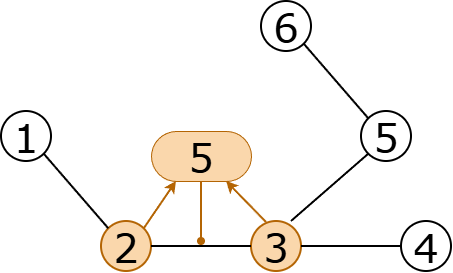
\includegraphics[width=4.0cm]{Figures/k_0.png}}
	%\hfill
	\subfloat[\centering]{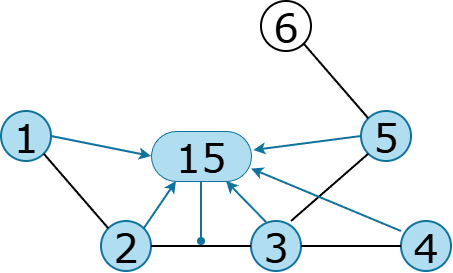
\includegraphics[width=4.0cm]{Figures/k_1.png}}
	\subfloat[\centering]{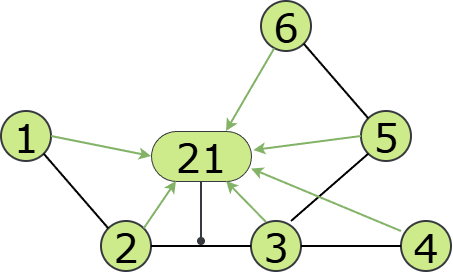
\includegraphics[width=4.0cm]{Figures/k_2.png}}
	%\hfill
	%\isPreprints{}{% This command is only used for ``preprints''.
	% \end{adjustwidth}
	%} % If the paper is ``preprints'', please uncomment this parenthesis.
	\caption{Illustration of target variable behavior across different k: (\textbf{a}) $k = 0$. (\textbf{b}) $k=1$. (\textbf{c}) $k=2$. \label{fig:k_hop}}
\end{figure}

\subsection{Proposed Architecture.} Experiments were conducted with various GNN architectures, including different
kinds of message-passing, GCN, GAT, and GraphSAGE \cite{hamilton2017inductive,
	kipf2017semisupervisedclassificationgraphconvolutional,
	veličković2018graphattentionnetworks} layers, as well as regularization methods
such as Dropout, LayerNorm, and GraphNorm. Ultimately, an architecture
utilizing an attention mechanism was proposed, demonstrating strong
performance. The constructed GNN consists of two main components:

\begin{enumerate}
	\item A \textbf{node encoder} using a sequence of GATv2 layers, LayerNorm, and ReLU
	      activation, aggregated via Jumping Knowledge with concatenation
	      \cite{brody2021attentive, xu2018representationlearninggraphsjumping}.
	\item An \textbf{edge attention layer} implementing multi-head attention over edges
	      sharing a common node, followed by LayerNorm and skip-connections.
\end{enumerate}

The main findings from the architecture search and ablation study were: first,
the use of spatial node coordinates ($x,y$) significantly improved prediction
quality; second, the attention mechanism was a key component regardless of the
complexity of the task; and third, the selected architecture outperformed all
others considered in learning local functional dependencies.

\subsection{Physically Modeled Dataset Generation}
To generate the dataset required for training the GNN, a thermohydraulic
simulation was employed to model the physical behavior of the DHN under various
operational and fault conditions. The heating network in the simulation is
represented as an oriented graph, where the nodes correspond to pipe junctions
and heat sources, and the edges represent pipeline branches with specified
geometric, thermal, and hydraulic parameters. Notably, to close the hydraulic
circuit, the end consumers are modeled as specialized edges connecting the
supply and return sub-networks; these consumer edges are assigned specific
local hydraulic resistance coefficients and heat transfer parameters to
simulate the pressure drop and thermal extraction of building's internal
heating system. The flow distribution within the network is governed by the
hydraulic circuit theory, requiring the simultaneous solution of mass and
momentum conservation equations \cite{vesterlund2015method}.

The hydraulic state is determined from conservation of mass at each node and a
momentum (head-loss) relation on each branch. Let branch $b=(i,j)$ connect
nodes $i$ and $j$, and let its positive direction be chosen from $i$ to $j$.
The unknown hydraulic variables are the nodal pressures $p_i$ and the branch
mass flow rates $m_b$, whose sign indicates the flow direction relative to the
branch orientation. In discrete graph form, nodal continuity is written as
\begin{equation}
	\sum_{b \in \mathcal{U}_i} \varepsilon_{ib} m_b = q_i,
\end{equation}
where $\mathcal{U}_i$ is the set of branches incident to node $i$, $\varepsilon_{ib}=\pm 1$
is the incidence sign determined by branch orientation, and $q_i$ represents the
external mass source or sink at the node.

The momentum conservation along each pipeline segment is described by the
nonlinear relation
\begin{equation}
	s_b |m_b| m_b = -\Delta p_b,
\end{equation}
where $\Delta p_b = p_j - p_i$ is the pressure drop across branch $b$, and $s_b$ is the
effective hydraulic resistance coefficient of the branch. In general, $s_b$ is determined
by the hydraulic properties of the branch and may include both distributed friction and
local hydraulic losses. In this case, the effective resistance can be written as
\begin{equation}
	s_b =
	\frac{1}{2 \rho_b A_b^2}
	\left(
	\lambda_b \frac{L_b}{D_b} + \xi_b
	\right),
\end{equation}
where $\lambda_b$ is the Darcy friction factor, $L_b$ is the branch length, $D_b$ is the
hydraulic diameter, $A_b$ is the cross-sectional area, and $\xi_b$ is the sum of local
hydraulic resistance coefficients.
In the present simulations, the Darcy friction factor was evaluated using the explicit
Altshul correlation,
\begin{equation}
	\lambda_b =
	0.11\left(
	\frac{\delta_b}{D_b}+\frac{68}{Re_b}
	\right)^{0.25},
\end{equation}
where $\delta_b$ is the equivalent roughness of the pipe wall, $\mu_b$ is the dynamic
viscosity, and
\begin{equation}
	Re_b = \frac{\rho_b |u_b| D_b}{\mu_b}
	= \frac{|m_b|D_b}{\mu_b A_b}
\end{equation}
is the branch Reynolds number. This explicit relation was used to avoid an additional
inner iteration for $\lambda_b$ within the global hydraulic pressure-correction procedure.

To solve these equations, the simulation employs a SIMPLE-like iterative
procedure. This algorithm utilizes an explicit equation for pressure
correction,
\begin{equation}
	\nabla \cdot (\kappa \nabla p') = \nabla \cdot m - q,
\end{equation}
where $p'$ is the pressure correction and
\begin{equation}
	\kappa_b = \frac{1}{s_b |m_b|}.
\end{equation}
The solver sequentially updates the nodal pressure field and branch mass flow rates through
iterations until strict mass-balance convergence is achieved across the entire network.

Thermal calculations are coupled to the hydraulic solution by evaluating
convective heat transport and thermal losses to the environment after hydraulic
calculation iteration. Heat loss from a pipe to ambient air is modeled by the
Newton--Richmann relation
\begin{equation}
	Q = \alpha F (t_b - t_{out}),
\end{equation}
where $\alpha$ is the overall heat transfer coefficient, $F$ is the pipe surface area, $t_b$
is the average water temperature within the pipe, and $t_{out}$ is the ambient outdoor
temperature. The average pipe temperature $t_b$ is calculated from the steady one-dimensional
energy balance with distributed heat loss,
\begin{equation}
	\label{eq:branch_temperature}
	t_b = t_{out} +
	\frac{\dot{m}_b c_p}{\alpha F}
	(t_1 - t_{out})
	\left[
		1 - \exp\left(
		-\frac{\alpha F}{\dot{m}_b c_p}
		\right)
		\right],
\end{equation}
where $\dot{m}_b$ is the branch mass flow rate, $c_p$ is the specific heat capacity, and
$t_1$ is the inlet temperature of the pipe.

Equation~\eqref{eq:branch_temperature} describes a steady branch-integrated
solution of the one-dimensional energy balance with distributed heat loss.
Under the quasi-stationary assumptions used in this work, the logarithmic mean
thermal driving force is applicable over a branch of arbitrary length, provided
that the mass flow rate, heat-transfer coefficient, ambient temperature, and
thermophysical properties are treated as constant or branch-averaged within
that branch. The branch length is therefore already accounted for through the
heat-transfer surface area $F$ and the exponential attenuation factor $\alpha
	F/(\dot{m}_b c_p)$, additional axial subdivision is not required to evaluate
the steady heat loss of a uniform branch. This formulation, however, does not
resolve thermal transport delays, hot-water-front propagation, or pipe-wall
thermal inertia. These effects are outside the scope of the present dataset,
where each sample represents a quasi-stationary operating regime used for fault
localization, and the sequential evolution of hydraulic and thermal states
during a transient process is not modeled.

At network nodes where multiple fluid streams intersect, perfect adiabatic
mixing is assumed, and the resulting nodal temperature is computed as the
mass-weighted average of the incoming flows. All thermal properties of the heat
carrier fluid, including density, dynamic viscosity, and specific heat
capacity, are dynamically updated during the iterations based on the local
fluid temperature.

To unify the hydraulic and thermal calculations, an iterative steady-state
simulation algorithm is used. The computational sequence starts by assigning
initial approximations of nodal pressures and temperatures from the network
boundary conditions. Based on these values, temperature-dependent
thermophysical properties of the fluid are evaluated and initial branch mass
flow rates are estimated. The core of the algorithm then enters an iterative
hydraulic loop: the branch mass flows are updated from an iterative solution of
the momentum conservation equations, after which a global pressure-correction
equation is solved to adjust the nodal pressure field and correct the branch
flows.

Once the hydraulic flow distribution is stabilized, the algorithm proceeds to
the thermal step and updates the temperature field; the fluid density,
viscosity, and heat capacity are then recalculated for each pipe using the
newly obtained local temperatures. The coupled iterations continue until the
predefined convergence criterion is satisfied; otherwise, the solver returns to
the hydraulic phase with updated thermophysical properties.

Using this simulation approach, a local segment of an urban DHN located in
Arkhangelsk Oblast, Russia, was modeled. The case study represents a compact
residential district served by a central heat source and includes consumer
stations together with the interconnecting supply and return pipeline
infrastructure. The resulting graph contains 187 nodes and 202 pipe segments.
\textcolor{blue}{Thus, the modeled object is a local hot-water supply/return
DHN segment rather than a complete city-wide heat-supply system; consumer
stations are heat sinks, and the source/sink symbols in Figure~\ref{fig:dhn}
denote the heat-source supply/return boundary nodes.}
The heat source is represented by boundary conditions: specified supply flow
rate and temperature, and fixed return pressure, while the boiler outlet
pressure is obtained within the hydraulic solution.

To provide a representative range of operating conditions, simulations followed
an operational temperature curve that maps outdoor ambient temperature to the
required source supply temperature and mass flow rate. Consumer heat demands
were also scaled according to the same curve. The outdoor temperature was
varied from $-34^{\circ}\mathrm{C}$ to $+10^{\circ}\mathrm{C}$ with
$1^{\circ}\mathrm{C}$ increments to define baseline environmental scenarios.

\textcolor{blue}{Therefore, the boundary conditions in the generated dataset
are scenario-dependent values defined by this operating curve rather than a
single fixed operating point; the ambient-temperature range specifies the load
envelope covered by the simulations.}

For each baseline scenario, a grid of operational states with various
modifications of baseline scenario, was generated, resulting in a final dataset
of 42570 samples. Natural data noise (environmental fluctuations and
measurement uncertainty) was simulated by applying random variations within
$5\%$ of heat transfer coefficient $\alpha$ on a randomly selected 10--20\%
subset of pipes. To emulate localized thermal degradation (e.g., insulation
failure or pipe flooding), a set of defect scenarios in which $\alpha$ was
increased in a single pipeline segment was generated. The defect location was
swept over all pipeline segments in the network, excluding consumer-modeling
pipes. Five defect severity levels were considered, corresponding to
\textcolor{blue}{increased heat transfer in the ranges 120--150\%, 150--170\%,
170--200\%, 200--300\%, and 300--400\% of the baseline $\alpha$ value.}

\textcolor{blue}{Consumer-modeling pipes are auxiliary graph edges that
connect the supply and return subnets through a consumer station and represent
consumer-side hydraulic resistance and heat extraction. They are not treated as
candidate distribution-pipeline fault classes in the present localization
task.}

\textcolor{blue}{In this formulation, a defect is not modeled as a mass leak:
	no water-loss term is added to the nodal mass-balance equation and the branch
	mass-flow equations remain closed. The fault corresponds to a local increase
	in heat transfer through the pipe wall/insulation. A true leakage case with
	water loss would require an additional mass source/sink term in the continuity
	equation and changed branch flows; this case is outside the scope of the
	current dataset.}

\textcolor{blue}{The dataset generation process produced the following samples for each temperature regime: 10 defect-free operational states and 935 defective states (5 simulations for each of the 187 pipes). Additionally, for each temperature, a reference sample without defects or noise was generated as a baseline. In total, the dataset contains 42,525 training samples (42,075 defective and 450 defect-free) plus 45 reference samples.}

\textcolor{blue}{When preparing the data for training, the full graph was split into supply and return subnets, resulting in 85,050 total samples: 42,075 with a defect in the considered subnet (49.5\%) and 42,975 without a defect (50.5\%) - the latter includes 42,075 samples from the opposite subnet plus 450 defect-free samples from each subnet. This balanced distribution between defective and non-defective samples was intentionally designed to ensure robust model training.}

\subsection{Stage 2: Application to DHN Fault Localization}\label{stage2}

% In Stage 1, to identify an architecture capable of effectively capturing data propagating from neighboring nodes, we conducted a series of experiments on synthetic data, framing the problem as edge-level regression. Having understood what a suitable GNN should look like, we moved on to fault localization in DHNs. Since the real-world graph data is extremely sparse, we reformulated the problem as multi-class classification. For this purpose, we modified the network by replacing the final regression layer with a classification head and adding a global pooling.

Stage 2 builds on the design choices and assumptions that worked well in Stage
1. In Stage 1, the objective was to verify the model's capacity to aggregate
information from multi-step ($k$-hop) neighborhoods by learning functional
dependencies from synthetic data (Equation \ref{k_sum}). This capability is
critical for DHN fault localization because physical disturbances, such as
pressure drops or temperature anomalies, propagate spatially through the
network. Consequently, the model must capture these local topological
dependencies to accurately trace the fault source.

Having understood what a suitable GNN should look like, we moved on to fault
localization in the DHN. \textcolor{blue}{To mimic realistic sparse monitoring,
	dynamic pressure and temperature values are retained only at 30 nodes: the
	heat-source supply and return nodes, and the supply/return connection points
	of the 14 consumers (2 nodes per consumer).} This configuration mirrors real-world
conditions where sensor coverage is sparse. Since edge-level regression is
impractical under such sparsity, we reformulated the problem as multi-class
classification. For this purpose, we adapted the architecture by replacing the
final regression layer with a classification head and introducing global
pooling.

We used a prepared dataset of 42,570 simulated operational states of a DHN,
represented as a graph with 187 nodes (junctions, consumers, source/sink) and
202 edges (pipes) illustrated in Figure~\ref{fig:dhn}. %Simulations covered 45 outdoor temperature regimes ($-33^\circ$C to $+10^\circ$C). For each temperature, scenarios included: a baseline (no defect), cases with noise (5\% variation in insulation), and cases with a single defective pipe (with five severity levels from 120\% to 400\% increased heat transfer).

\begin{figure}[H]
	%\isPreprints{\centering}{} % Only used for preprints
	\begin{adjustwidth}{-\extralength}{0cm}
		\centering
		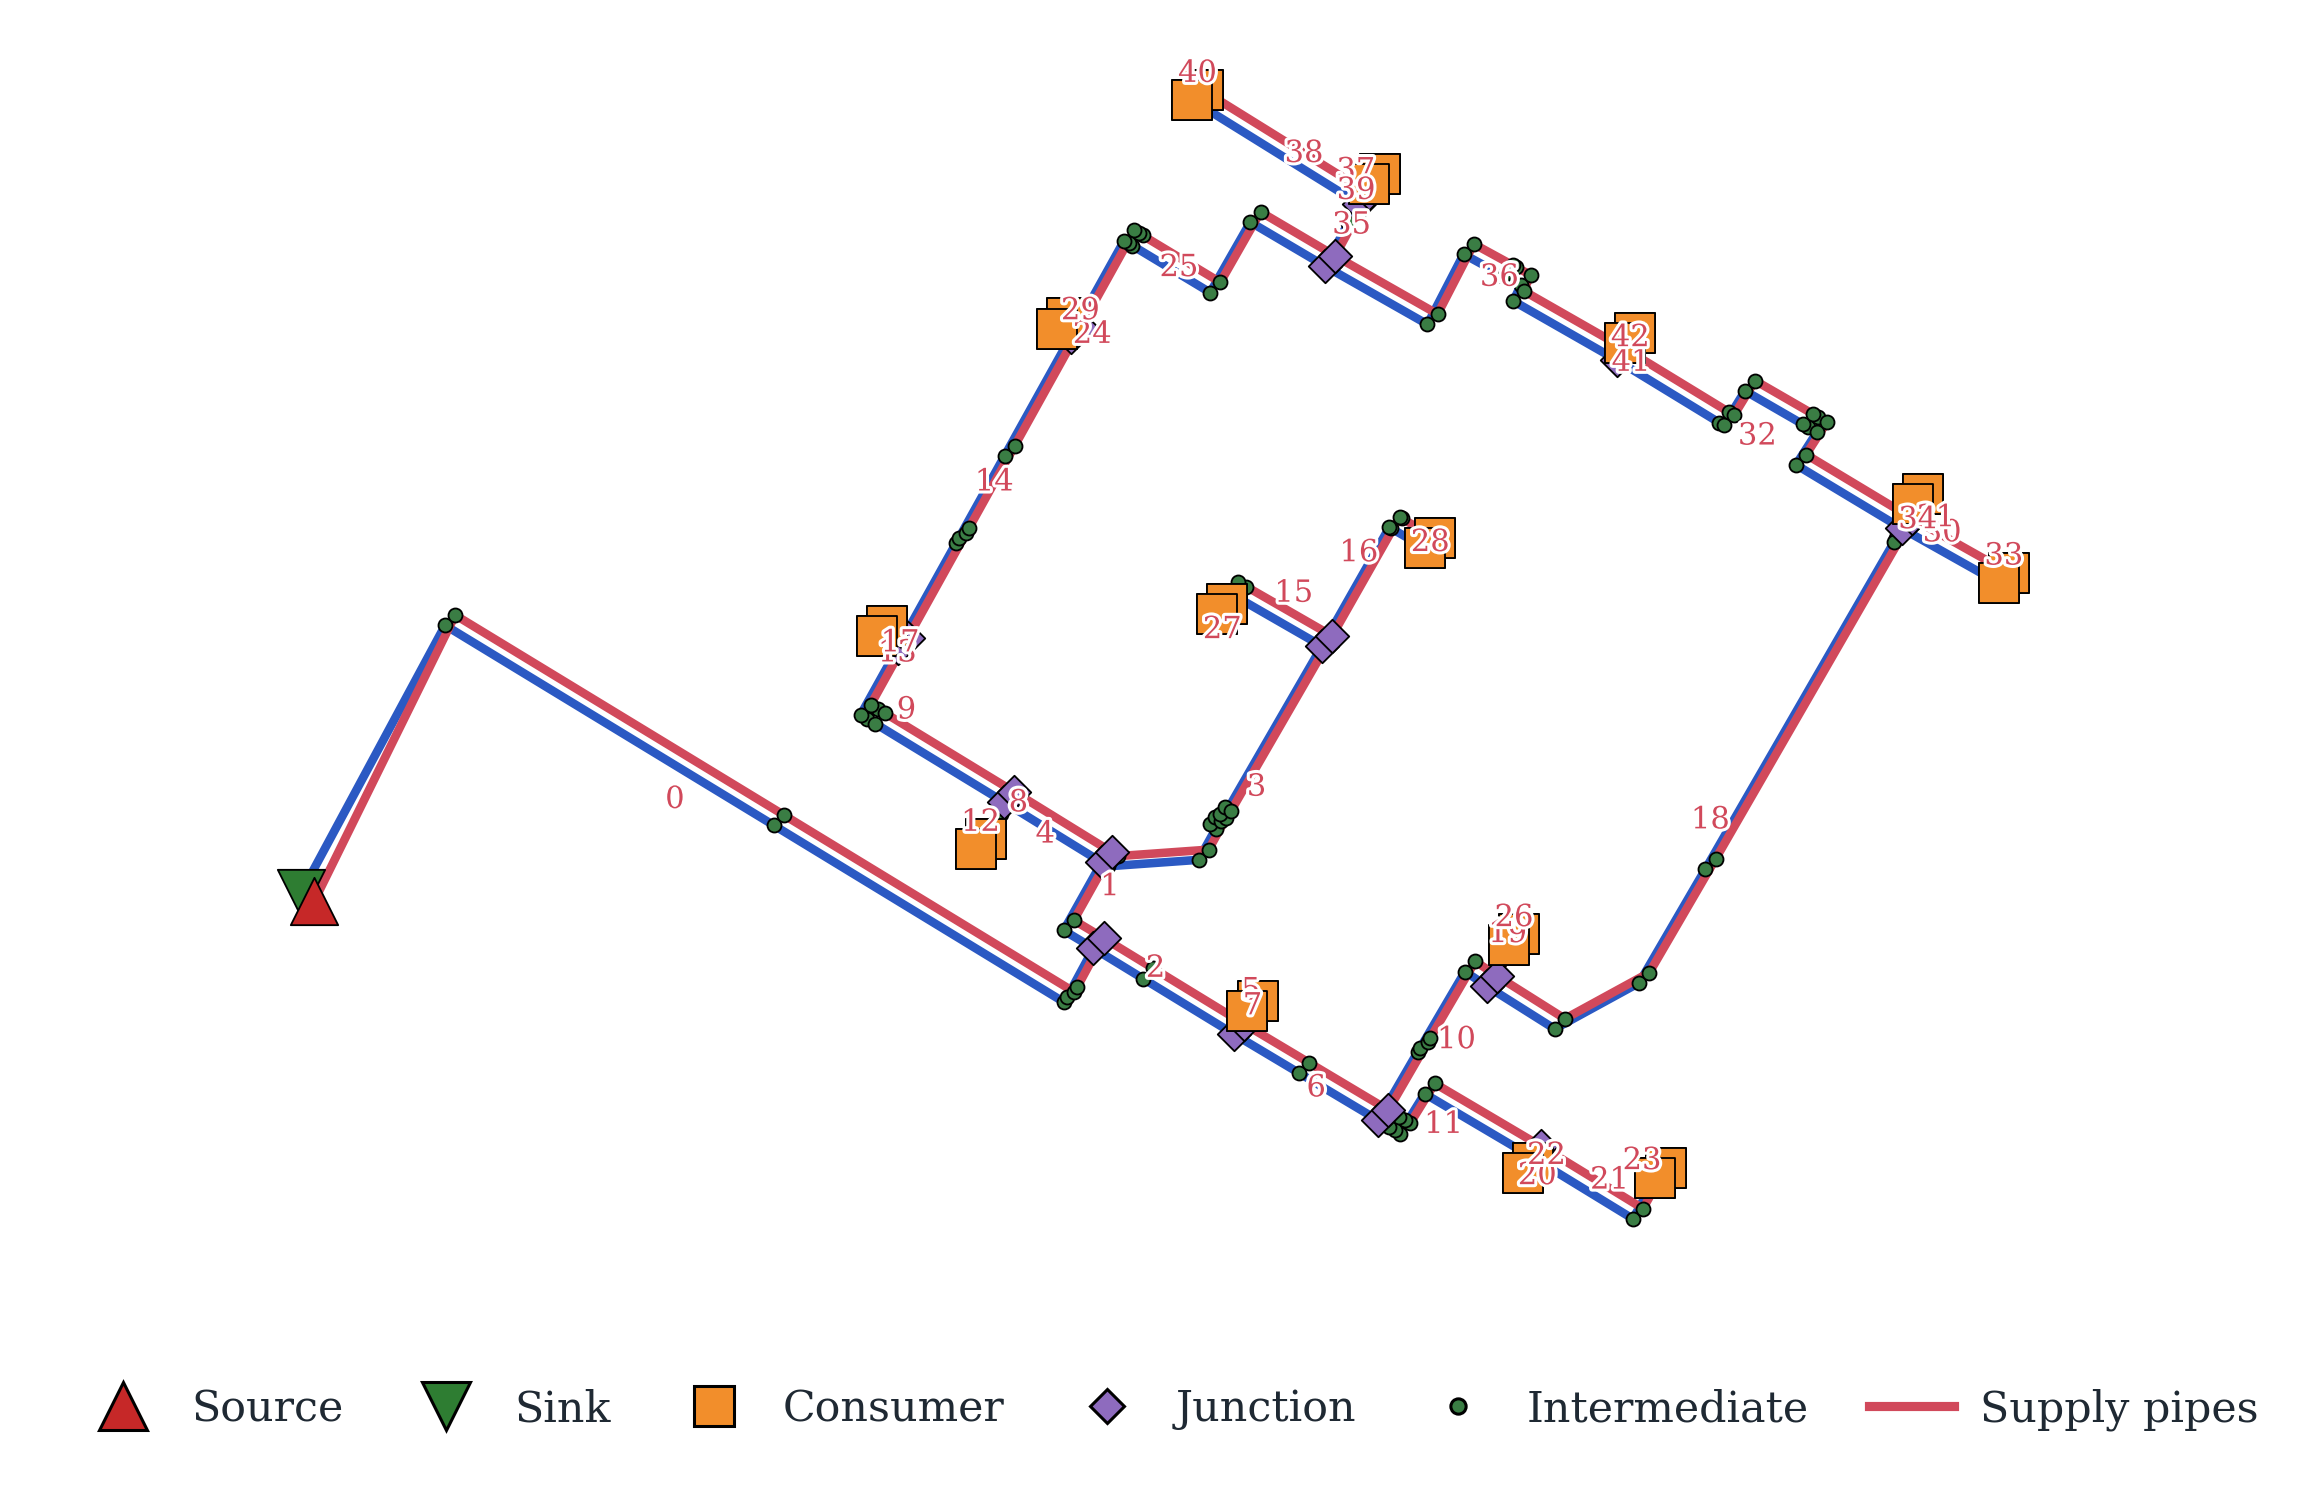
\includegraphics[width=16.0 cm]{Figures/dhn_example_new.png}
	\end{adjustwidth}
	\caption{An illustration of the district heating network.\label{fig:dhn}}
\end{figure}

The following node features were used for model training:
\begin{itemize}
	\item Local $x$, $y$ coordinates of the node.
	\item Node type -- source, sink, or pipe junction.
	\item Pressure at the node -- a dynamic parameter.
	\item Temperature at the node -- a dynamic parameter.
\end{itemize}
The following pipe (edge) features were used:
\begin{itemize}
	\item Pipe diameter.
	\item Pipe length.
	\item Pipe type -- supply, return, or consumer line.
\end{itemize}
Additionally, the outdoor air temperature was used as an input parameter.

The data preprocessing pipeline consists of the following steps:
\renewcommand{\labelenumii}{\arabic{enumi}.\arabic{enumii}}
\renewcommand{\labelenumiii}{\arabic{enumi}.\arabic{enumii}.\arabic{enumiii}}
\renewcommand{\labelenumiv}{\arabic{enumi}.\arabic{enumii}.\arabic{enumiii}.\arabic{enumiv}}
\begin{enumerate}
	\item Splitting the large heating network graph into two intersecting subgraphs --
	      the supply and return subnets. These are formed by selecting all supply pipes,
	      return pipes, and consumer pipes along with their incident vertices in the
	      graph. These components have similar structures, as supply and return pipes are
	      physically co-located.
	\item Loading the data required for training, including global parameters such as
	      outdoor air temperature and boiler plant temperatures, which are duplicated
	      into separate tables.
	      \begin{enumerate}
		      \item A numerical identifier is added to each edge in the graph, indicating which
		            graph section the edge belongs to after partitioning. For each graph, a class
		            (numerical label) is assigned -- the index of the section containing the
		            defective edge (or a separate class if no defects are present).
		      \item The partitioning logic is as follows: edges belong to the same section if and
		            only if they form a direct path between two key vertices. A vertex is
		            considered a key vertex if it is a consumer vertex (incident to consumer
		            pipes), a boiler plant vertex (heat source or sink), or a junction vertex (with
		            in-degree + out-degree > 2).
		      \item Adding dynamic parameters (readings from temperature and pressure sensors) to
		            the graph vertices corresponding to consumers and the boiler plant (30 out of
		            187 vertices in total).
	      \end{enumerate}
	\item Transforming the raw data into a set of tabular representations.
	\item Estimating normalization parameters and scaling three groups of features (the
	      two heating network components and the global parameters) to zero mean and unit
	      standard deviation based on the training set.
	\item Applying normalization to all tabular data.
	\item Converting the normalized tabular data into graph objects used by the model.
\end{enumerate}

The core architecture from Stage 1 was adapted for classification as
illustrated in Figure~\ref{fig:arch}:
\begin{itemize}
	\item The final edge feature representations, enhanced by the node encoder and edge
	      attention blocks, were concatenated with their transformed versions from all
	      attention layers.
	\item A global pooling layer aggregated edge features into a single graph-level
	      representation.
	\item A linear classifier layer mapped this representation to logits over the
	      classes.
\end{itemize}

\begin{figure}[H]
	%\isPreprints{\centering}{} % Only used for preprints
	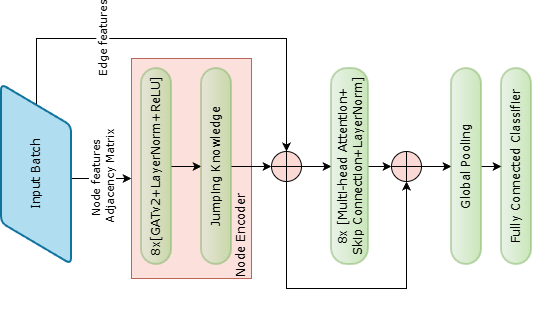
\includegraphics[width=10.0 cm]{Figures/architecture_horizontal.png}
	\caption{An illustration of the architecture of our GNN.\label{fig:arch}}
\end{figure}
\unskip

\subsection{Training.}

The model was trained for 100 epochs with a batch size of 16 graph pairs. The
dataset was split into training, validation, and test sets with a ratio of
70:15:15. \textcolor{blue}{We conducted 3-fold cross-validation, obtaining
	consistent accuracy scores (0.913±0.011, averaged between two subnets) across
	folds, confirming that the results do not depend on a particular data split.}
\textcolor{blue}{The split was performed randomly over generated operational
	states; therefore, outdoor-temperature regimes and severity ranges may be
	represented in all subsets. The evaluation thus measures interpolation across
	fault locations and operating states within the simulated operating envelope,
	rather than extrapolation to completely unseen climate regimes.}

The model was optimized using Adam \cite{kingma2015adam}. The initial learning rate was set to
$10^{-3}$, with $\beta = (0.9, 0.99)$, $\varepsilon = 10^{-8}$, and weight
decay $\lambda = 10^{-6}$. The learning rate was reduced exponentially each
epoch down to $10^{-6}$ using a StepLR scheduler with a step size of $1$ and
$\gamma = (10^{-6}/10^{-3})^{1/100} \approx 0.933254$.

The loss function was multi-class cross-entropy (CrossEntropyLoss) with label
smoothing ($\varepsilon=0.1$) and class weighting applied. The model
hyperparameters are listed in Table~\ref{tab:par}.

\begin{table}[H]
	\centering
	\begin{tabularx}{\textwidth}{CCC}
		\toprule
		\textbf{Parameter}              & \textbf{Value}         \\
		\midrule
		Node encoder layer dimension    & 128                    \\
		\hline
		Edge attention layer dimension  & 128                    \\
		\hline
		Number of node encoder layers   & 8                      \\
		\hline
		Number of edge attention layers & 8                      \\
		\hline
		Number of attention heads       & 8                      \\
		\hline
		Jumping knowledge mode          & \texttt{concatenation} \\
		\bottomrule
	\end{tabularx}
	\caption{Model Hyperparameters. \label{tab:par}}
\end{table}

\begin{figure}[H]
	\centering
	\subfloat[\centering Cross-entropy loss]{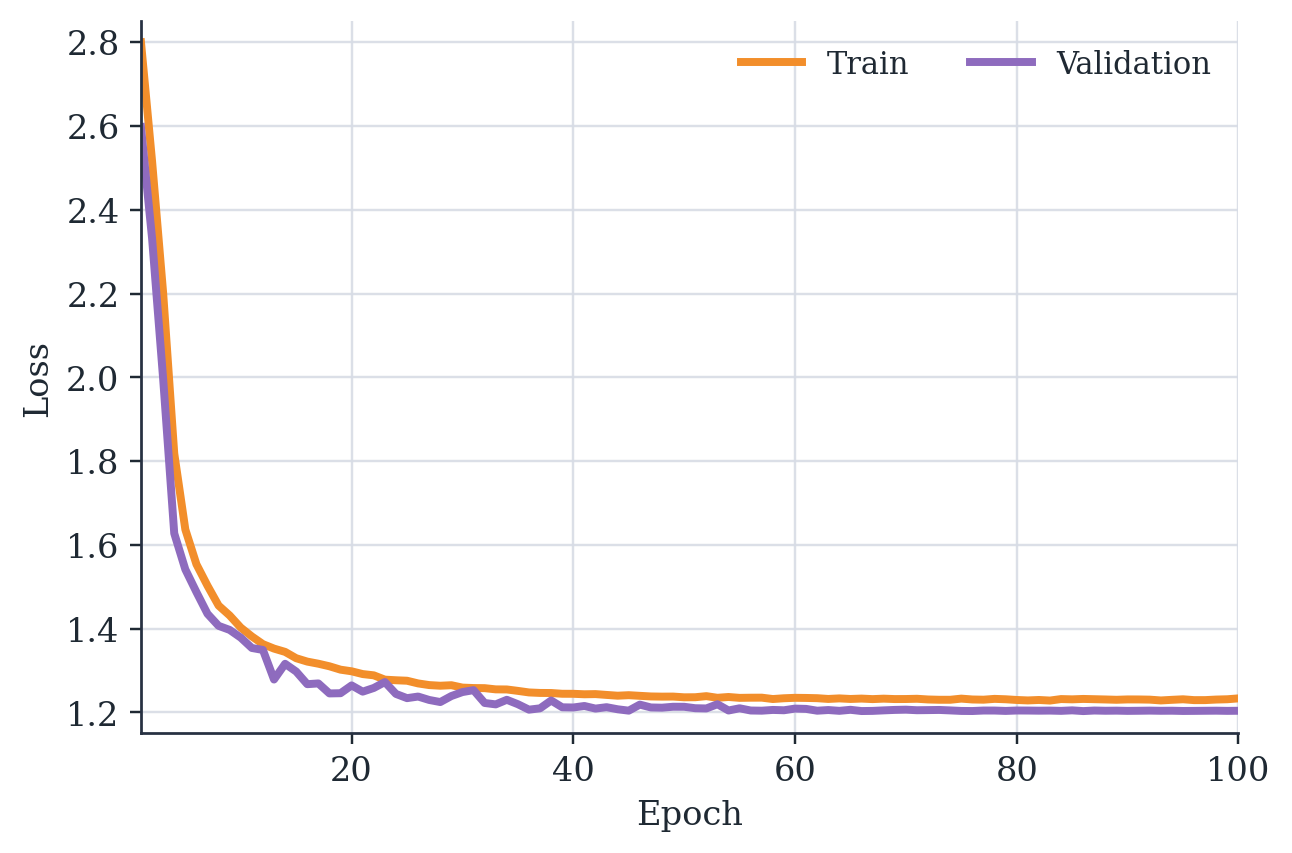
\includegraphics[width=0.48\textwidth]{Figures/Loss_combined.png}}
	\hfill
	\subfloat[\centering Accuracy]{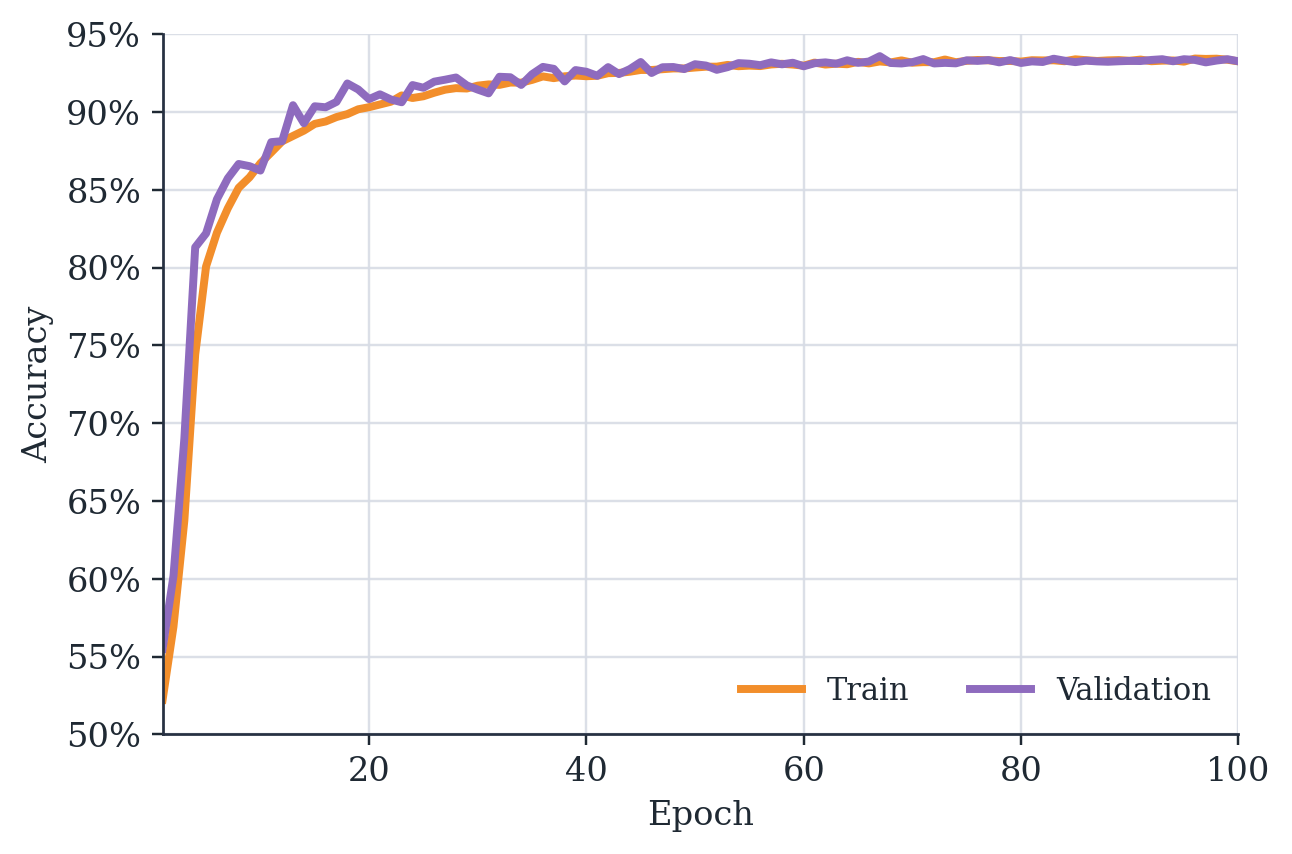
\includegraphics[width=0.48\textwidth]{Figures/Accuracy_combined.png}}
	\caption{Training vs. validation performance over epochs. \label{fig:loss_curves}}
\end{figure}

\subsection{Implementation}
All models were implemented using Python 3.12, PyTorch 2.4.1, and the PyTorch
Geometric 2.6.1 library.

%%%%%%%%%%%%%%%%%%%%%%%%%%%%%%%%%%%%%%%%%%
\section{Results and Discussion}

\subsection{Main Results}
The performance of the proposed GNN architecture was evaluated using the
physically modeled dataset described in Section \ref{stage2}. To ensure a
robust assessment of generalization, the model was trained using the Adam
optimizer, with convergence observed after approximately 50 epochs as indicated
by the stabilization of the validation loss on Figure \ref{fig:loss_curves}.

Table \ref{tab:main_res} presents the results achieved by our model on the test
dataset. The reported number of classes (30) includes both the specific fault
locations across the network sections and an additional class representing the
normal operating state ("no defect"). The mean Accuracy and Macro F1 scores
exceeding 90\% demonstrate that the model exhibits strong predictive
performance on sparse data, successfully capturing graph dependencies and
effectively handling the classification task. \textcolor{blue}{For a given
	class, precision is the fraction of predictions assigned to that class that
	are correct, while recall is the fraction of true samples of that class that
	are detected. The F1-score is their harmonic mean,
	$F1=2\cdot(\mathrm{precision}\cdot\mathrm{recall})/
		(\mathrm{precision}+\mathrm{recall})$. Macro F1 is the unweighted average
	of per-class F1 values and is therefore sensitive to performance on rare
	classes instead of being dominated by larger classes.}

\begin{table}[H]
	\centering
	\begin{tabularx}{\textwidth}{lCCCC}
		\toprule
		\multirow{2}{*}{\textbf{Model}} & \multicolumn{2}{c}{\textbf{Supply Subnet}} & \multicolumn{2}{c}{\textbf{Return Subnet}}                                         \\
		\cmidrule(lr){2-3} \cmidrule(lr){4-5}
		                                & \textbf{Accuracy}                          & \textbf{Macro F1}                          & \textbf{Accuracy} & \textbf{Macro F1} \\
		\midrule
		\multicolumn{5}{c}{\textbf{Baseline models}}                                                                                                                      \\
		\midrule
		Random Forest                   & 0.828                                      & 0.567                                      & 0.623             & 0.220             \\
		Hist. Gradient Boosting         & 0.829                                      & 0.591                                      & 0.675             & 0.379             \\
		MLP                             & 0.867                                      & 0.711                                      & 0.646             & 0.266             \\
		\midrule
		\multicolumn{5}{c}{\textbf{Proposed topology-aware model}}                                                                                                        \\
		\midrule
		GNN                             & \textbf{0.960}                             & \textbf{0.930}                             & \textbf{0.910}    & \textbf{0.869}    \\
		\midrule
		Number of classes               & \multicolumn{2}{c}{30}                     & \multicolumn{2}{c}{30}                                                             \\
		Number of samples               & \multicolumn{2}{c}{6380}                   & \multicolumn{2}{c}{6380}                                                           \\
		\bottomrule
	\end{tabularx}
	\caption{Performance comparison between baseline models and the proposed GNN on the fault localization task. The GNN substantially outperforms all topology-agnostic baselines, particularly on the return subnet and the Macro F1 metric.}
	\label{tab:main_res}
\end{table}

The observed performance discrepancy between the supply (0.960) and return
(0.910) subnets aligns with the physical characteristics of the system. The
return pipeline has a narrower range of dynamic values (temperature/pressure).
Since the fluid has already cooled and pressure has dropped, the relative
impact of a defect is smaller compared to the background noise.

To interpret the model's errors, we aimed to understand how far the predictions
deviate from the ground truth when the model misclassifies (in terms of graph
distance). For this purpose, we introduce a "distance confusion matrix" in
Figure \ref{fig:dist_cm}. The x-axis represents the true fault location (graph
section), while the y-axis shows the topological distance between the predicted
and true sections. Each cell indicates the proportion of predictions falling at
a given distance from the true class. Perfect predictions would yield a
horizontal line at distance 0 with value 1.0.

\begin{figure}[H]
	%\isPreprints{}{% This command is only used for ``preprints''.
	\begin{adjustwidth}{-\extralength}{0cm}
		\centering
		%} % If the paper is ``preprints'', please uncomment this parenthesis.
		\subfloat[\centering]{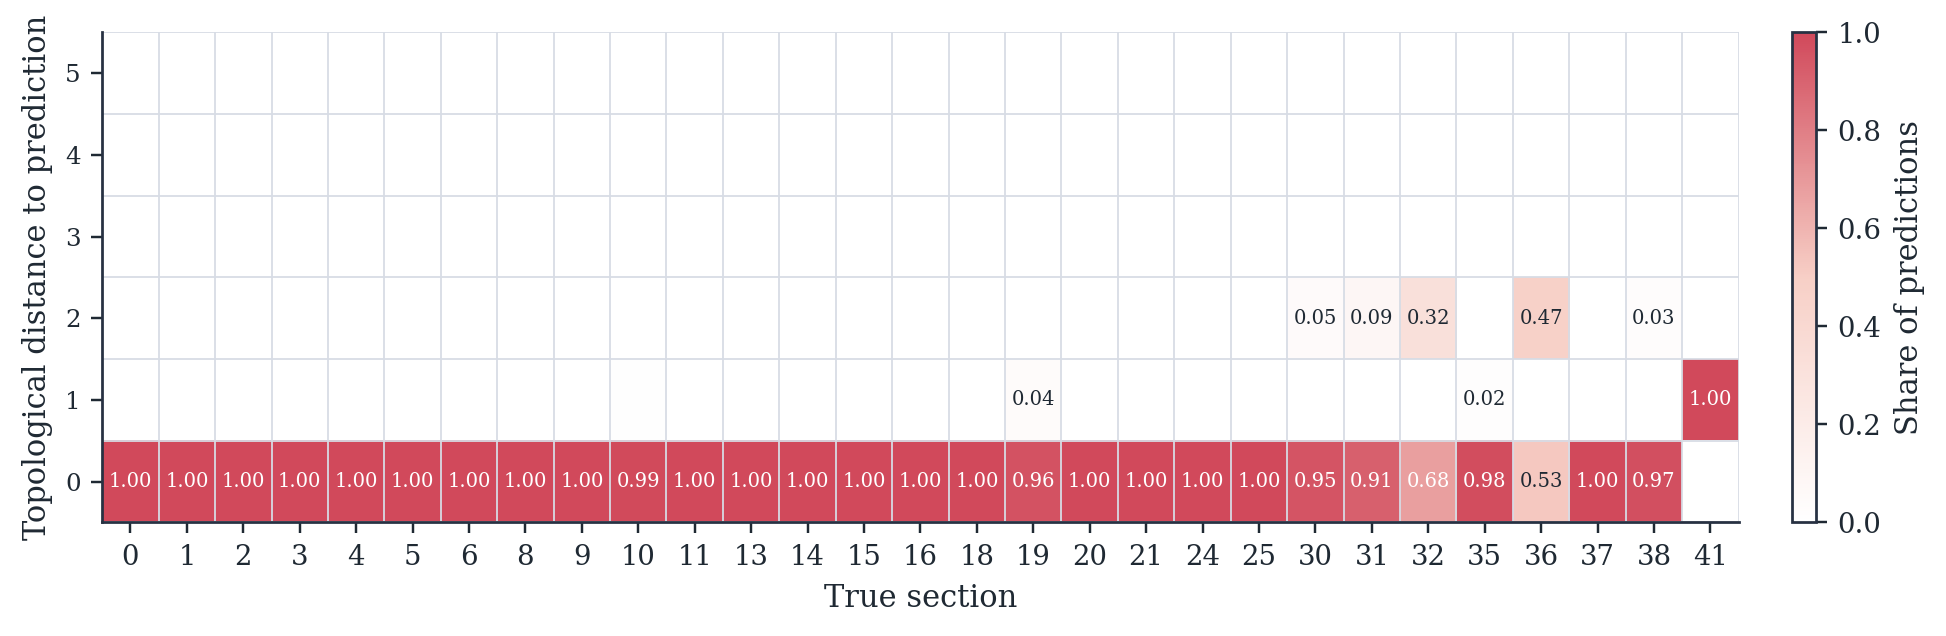
\includegraphics[width=16.0cm]{Figures/fwd_result_distance_confusion_matrix_transposed.png}}
		%\hfill
		\\
		\subfloat[\centering]{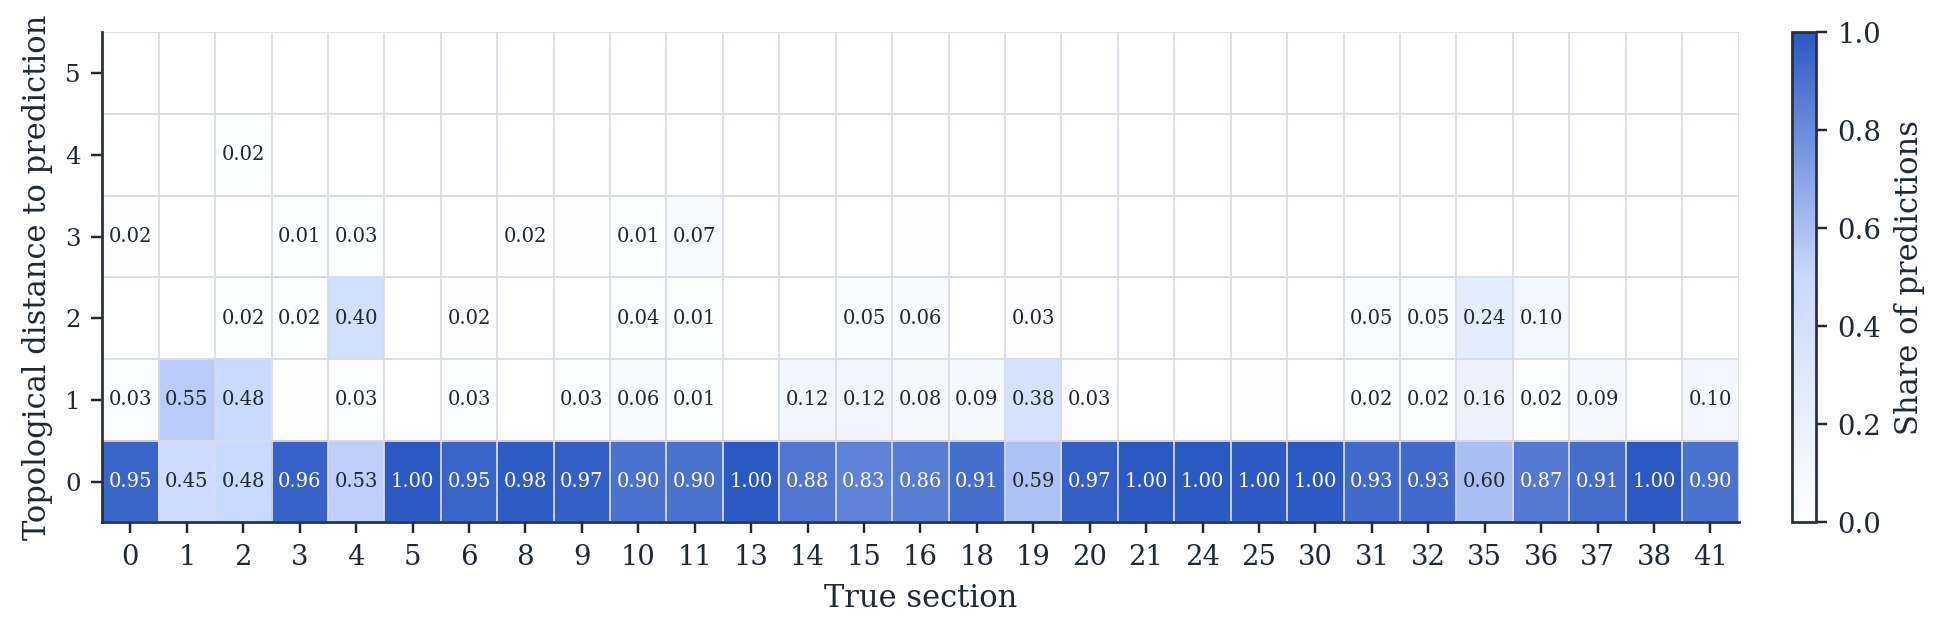
\includegraphics[width=16.0cm]{Figures/bwd_result_distance_confusion_matrix_transposed.png}}
		%\hfill
		%\isPreprints{}{% This command is only used for ``preprints''.
	\end{adjustwidth}
	%} % If the paper is ``preprints'', please uncomment this parenthesis.
	\caption{Distance confusion matrices: (\textbf{a}) Supply subnet. (\textbf{b}) Return subnet. \label{fig:dist_cm}}
\end{figure}

\textcolor{blue}{For segment 41, the value 1.0 at nonzero distance means that
	all 43 test samples belonging to this segment were assigned to another
	section. Segment 41 consists of a single pipe connecting a consumer to a
	branching node, resulting in fewer training examples compared to segments
	containing multiple pipes (N pipes \texttimes{} 225 defective samples per
	pipe). Additionally, segment 41 is topologically the farthest from the heat
	source among supply-side segments; temperature and pressure signals are
	attenuated, making the defect less pronounced. Consequently, the model
	misclassifies faults from segment 41 as belonging to neighbouring segments 32
	or 36, each of which comprises more pipes. The confusion matrix therefore
	indicates a local ambiguity among segments 32, 36, and 41 rather than random
	class substitutions. These sections are located in the most remote part of the
	supply subnet relative to the heat source, where pressure and temperature
	disturbances are weaker; this remoteness explains why defects in these
	segments are harder for the model to distinguish.}

Notably, the distribution of errors in Figure \ref{fig:dist_cm} demonstrates a
strong bias towards local mistakes. We observe that the error mass is heavily
concentrated within a topological distance of 1–2 sections, with negligible
occurrences of errors beyond that distance (relative to the network diameter of
12). Because heat loss and pressure drop affect neighboring segments, the model
correctly identifies the neighborhood of the fault even if it misassigns the
specific pipe edge. From an operational standpoint, this suggests that even in
cases of misclassification, the model effectively narrows the search area to
the vicinity of the actual fault. \textcolor{blue}{In practical terms, this
means that the initial inspection area can be limited to the predicted section
and its one- to two-section topological neighbourhood, before using additional
field diagnostics to identify the exact pipe edge.}

\textcolor{blue}{To complement the hop-based analysis, we also evaluated the
	metric localization error along the pipe network. For each prediction, the
	representative predicted position was taken as the midpoint of the predicted
	graph section, and the true position was taken as the midpoint of the defective
	pipe. The distance was then computed along the shortest path in the network
	using pipe lengths as edge weights. Figure~\ref{fig:metric_dist} shows that
	the physical-distance analysis is consistent with the topological-distance
	result: most correct and near-correct predictions remain spatially close to
	the true defect, while the largest errors are concentrated in the same
	problematic regions identified by the confusion matrices.}

\begin{figure}[H]
	\begin{adjustwidth}{-\extralength}{0cm}
		\centering
		\subfloat[\centering]{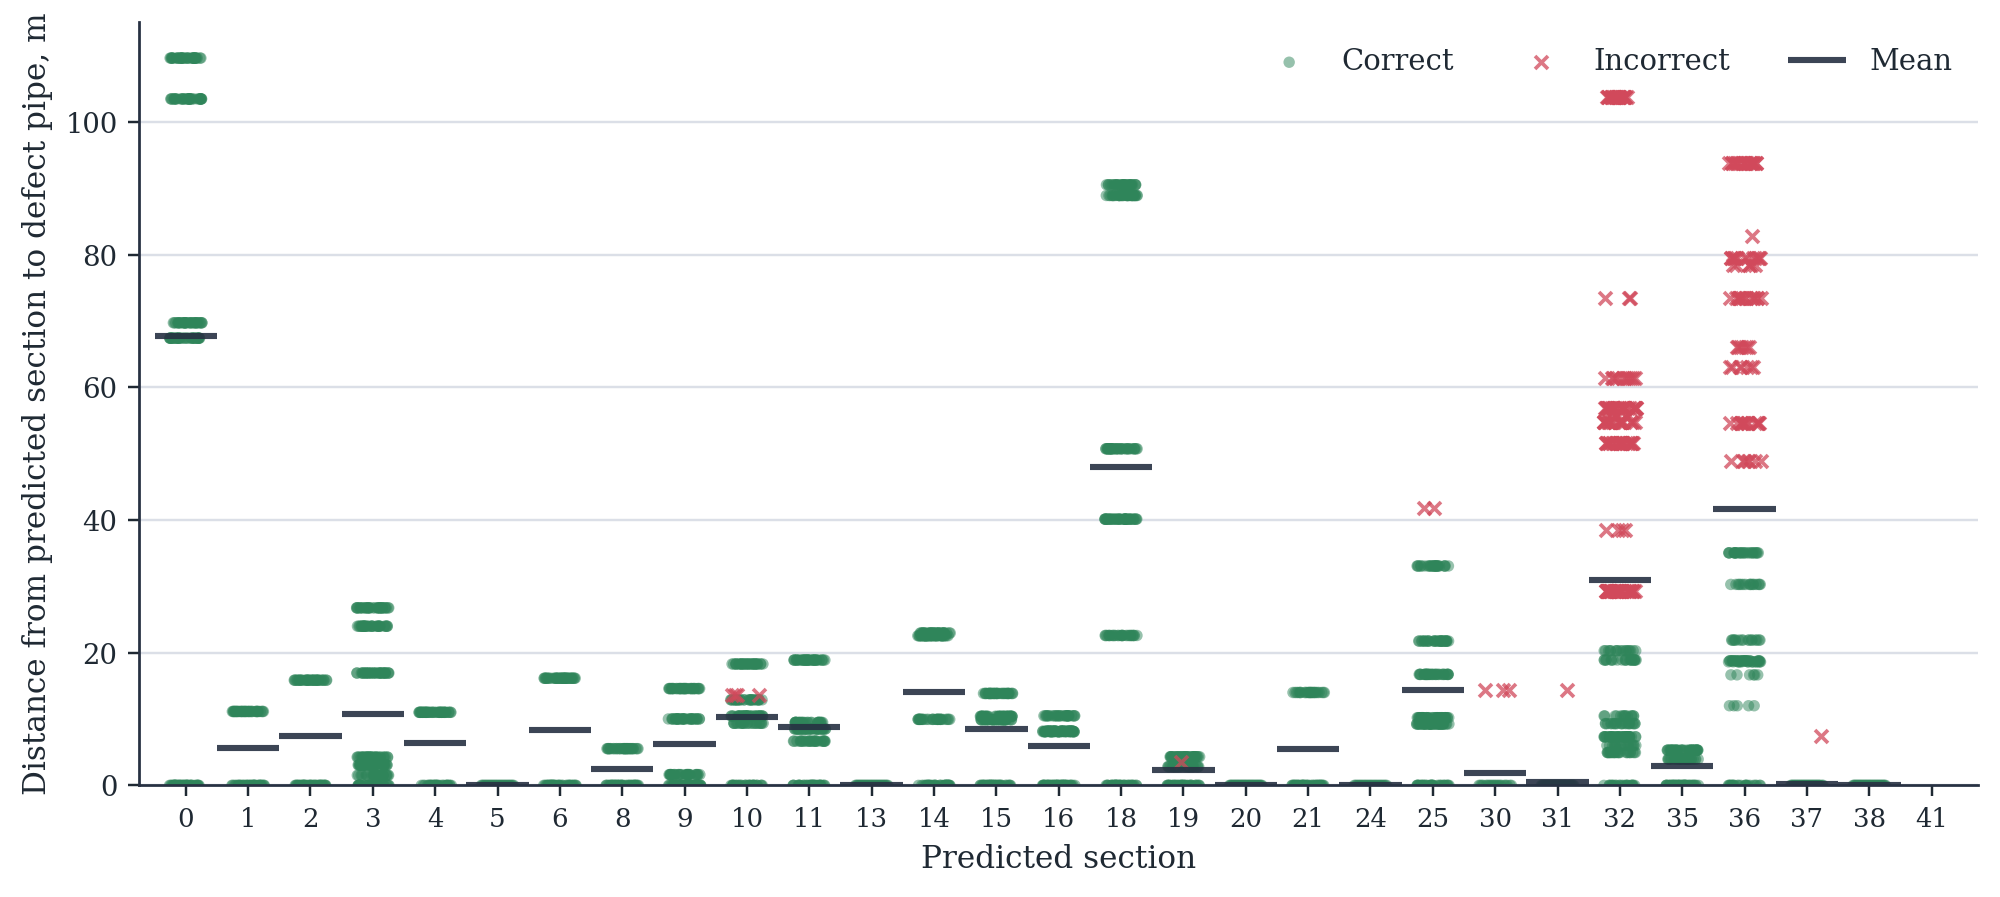
\includegraphics[width=16.0cm]{Figures/fwd_result_metric_distance_scatter.png}}
		\\
		\subfloat[\centering]{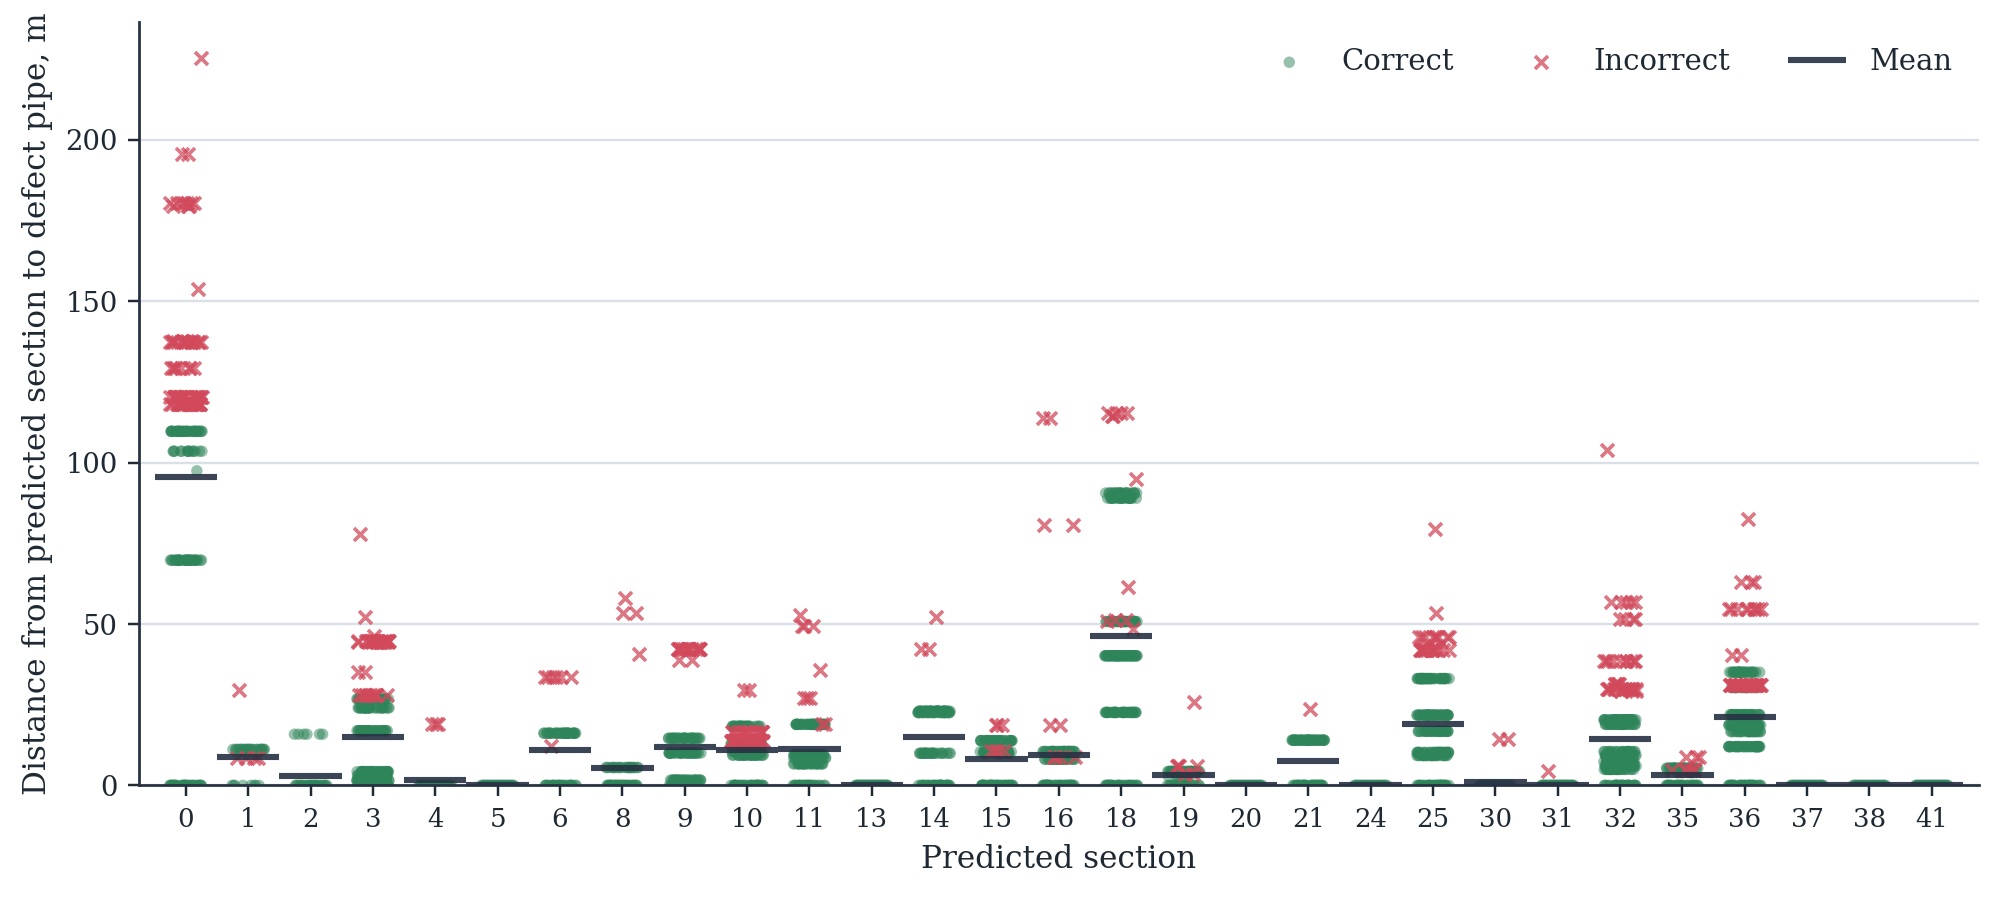
\includegraphics[width=16.0cm]{Figures/bwd_result_metric_distance_scatter.png}}
	\end{adjustwidth}
	\caption{Metric localization error measured along the pipe network: (\textbf{a}) Supply subnet. (\textbf{b}) Return subnet. Green points correspond to correctly classified samples, red crosses correspond to misclassified samples, and the dark horizontal marks show the mean distance for each predicted section. \label{fig:metric_dist}}
\end{figure}

\begin{figure}[H]
	\begin{adjustwidth}{-\extralength}{0cm}
		\centering
		\subfloat[\centering Class distribution]{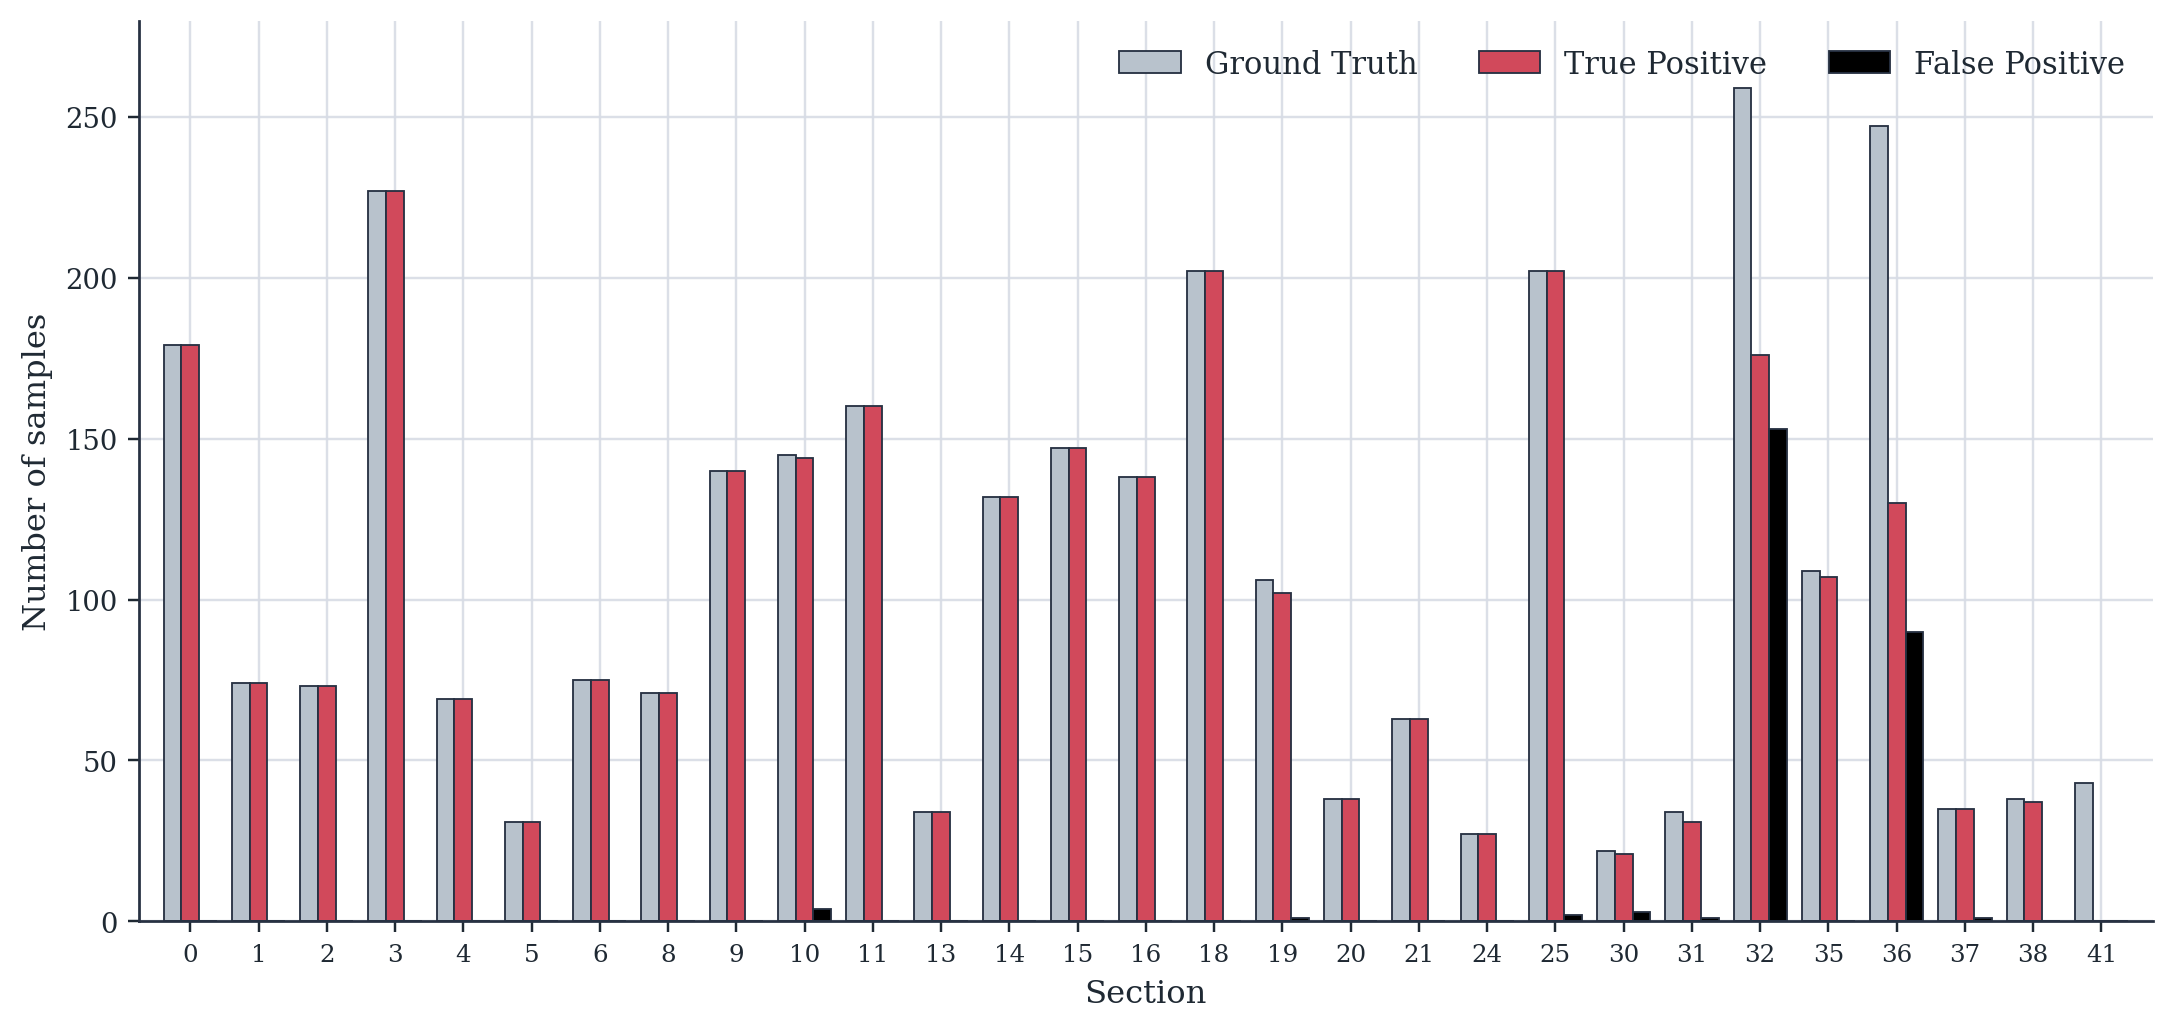
\includegraphics[width=15.5cm]{Figures/fwd_result_class_distribution_split.png}}
		\\
		\subfloat[\centering Normalized confusion matrix]{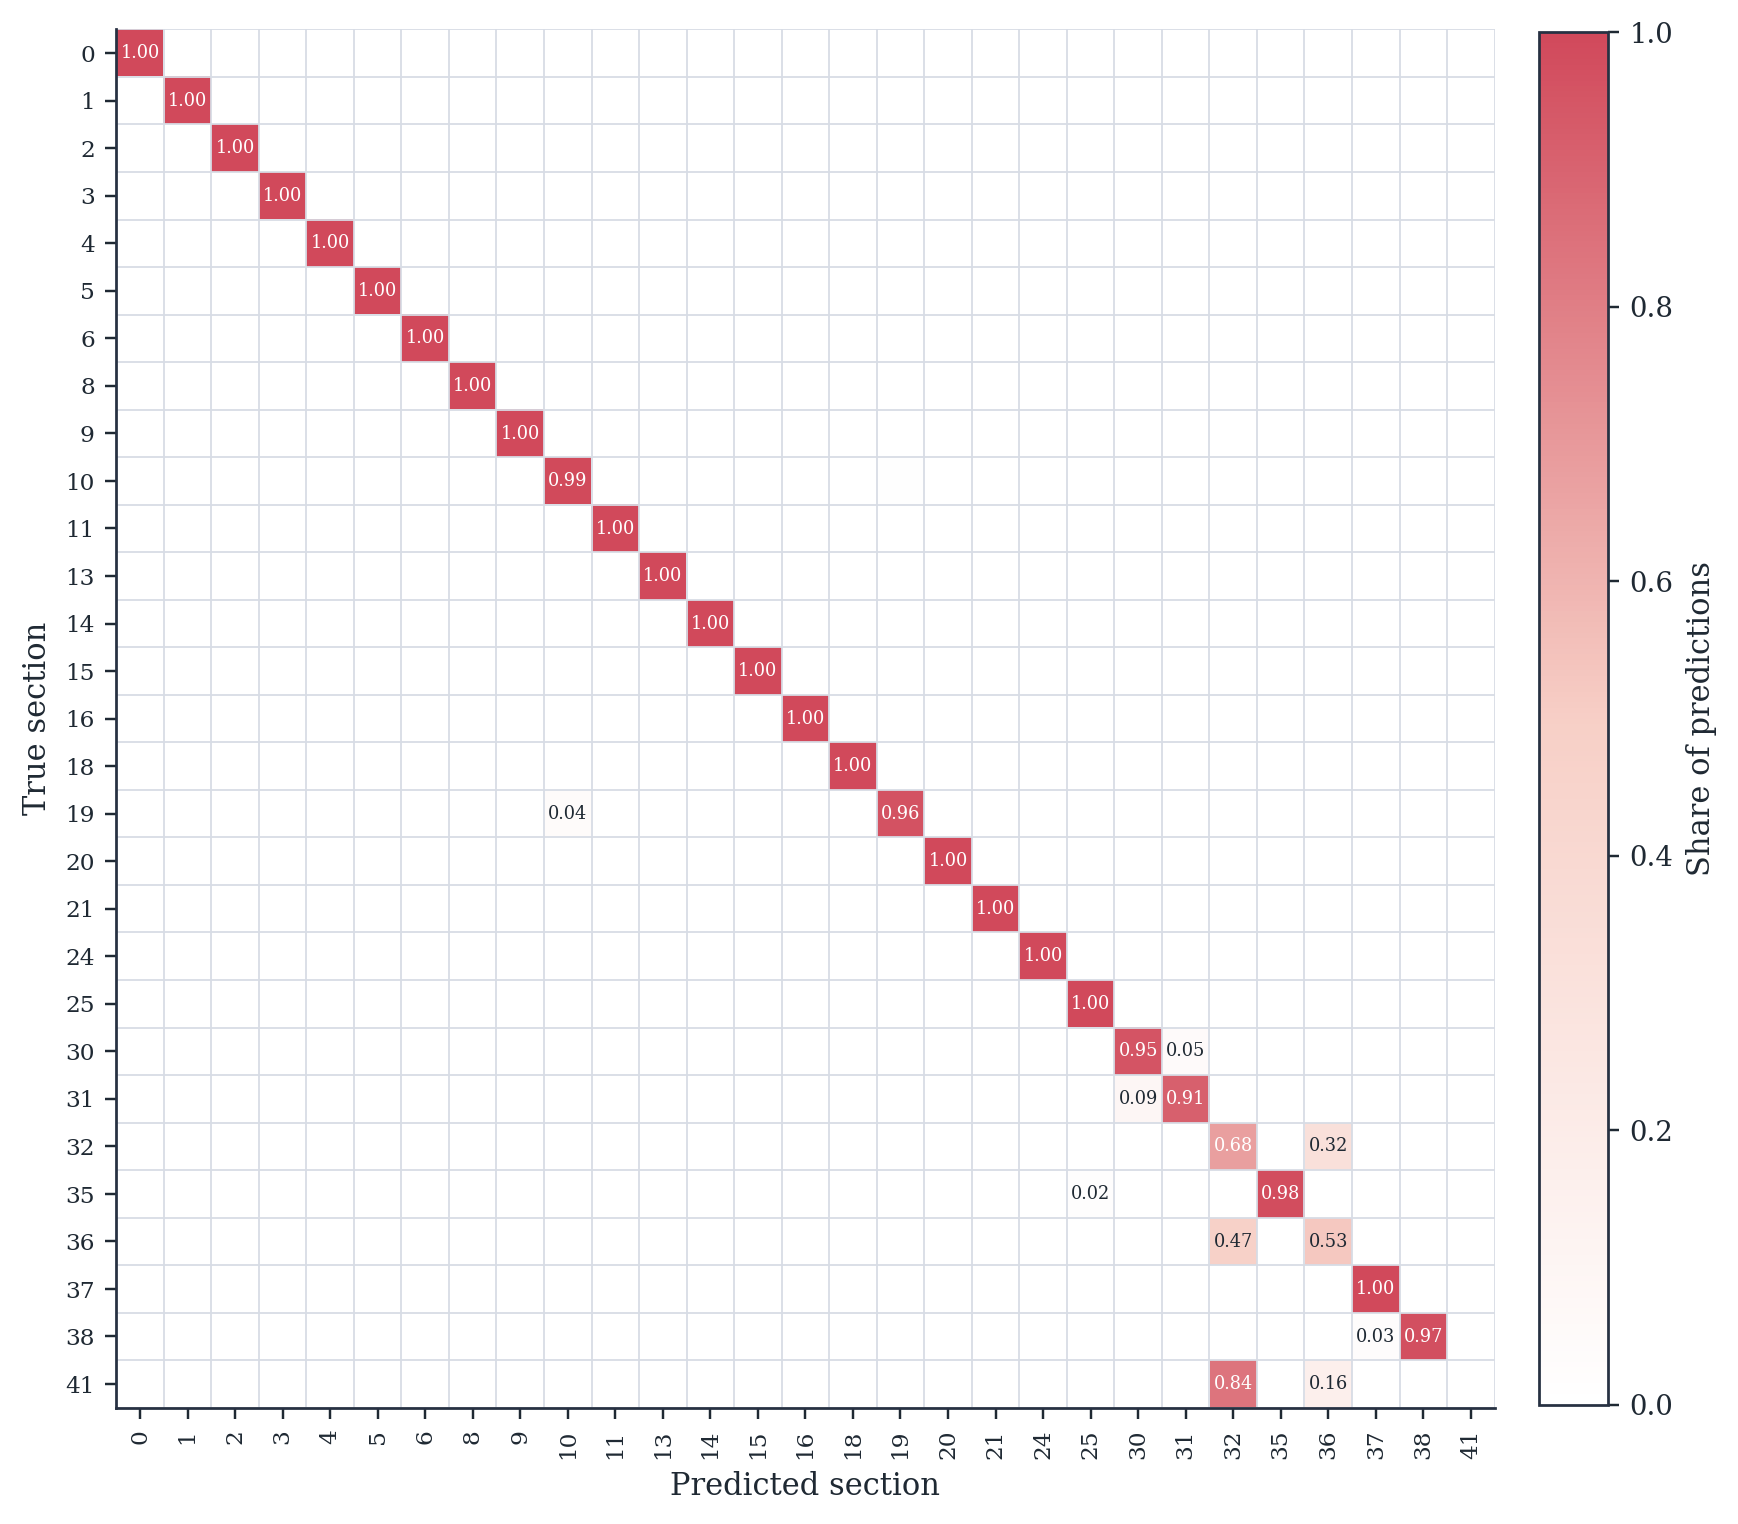
\includegraphics[width=15.5cm]{Figures/fwd_result_confusion_matrix_normalized.png}}
	\end{adjustwidth}
	\caption{Supply-subnet diagnostics, excluding the "no defect" class: (\textbf{a}) distribution of predicted classes and (\textbf{b}) normalized confusion matrix.
		\label{fig:supply_distribution_confusion}}
\end{figure}

\begin{figure}[H]
	\begin{adjustwidth}{-\extralength}{0cm}
		\centering
		\subfloat[\centering Class distribution]{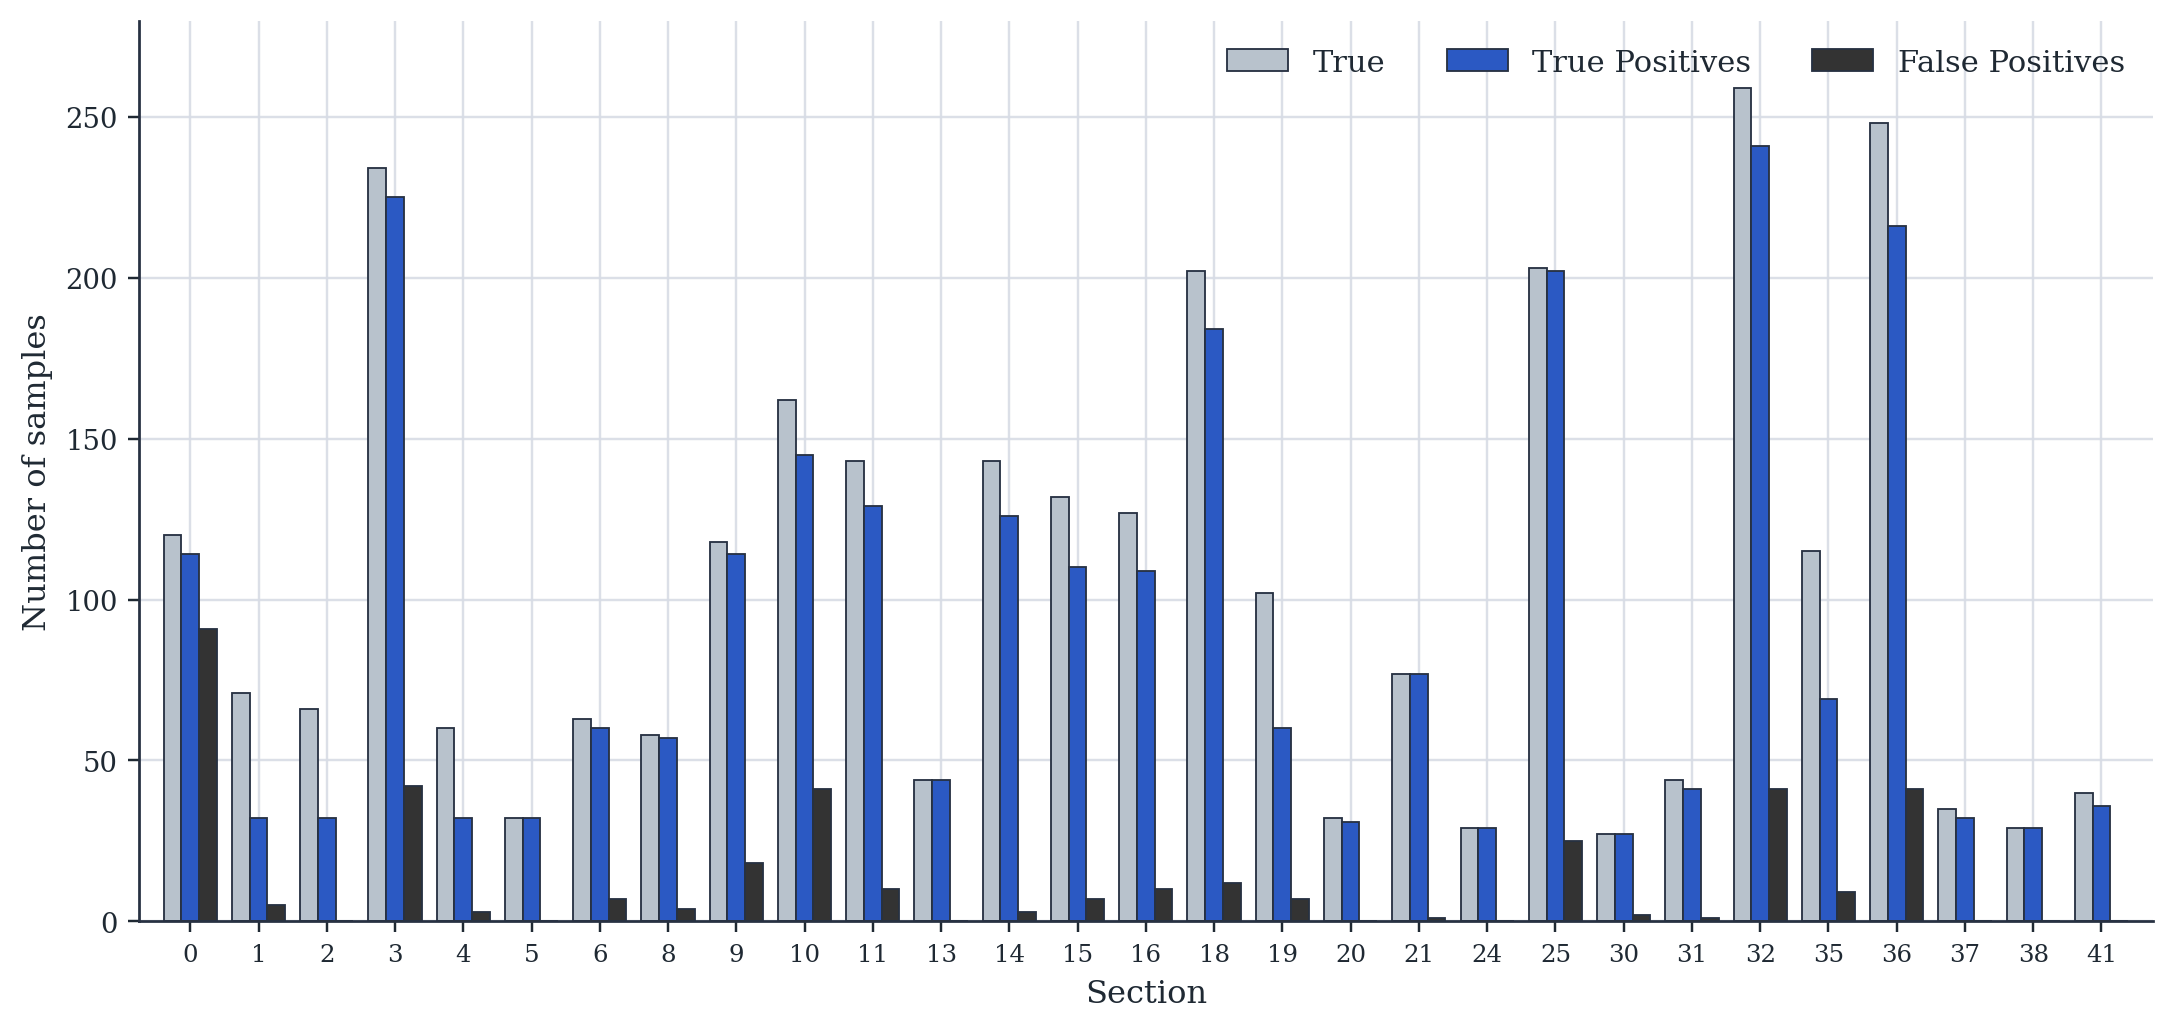
\includegraphics[width=15.5cm]{Figures/bwd_result_class_distribution_split.png}}
		\\
		\subfloat[\centering Normalized confusion matrix]{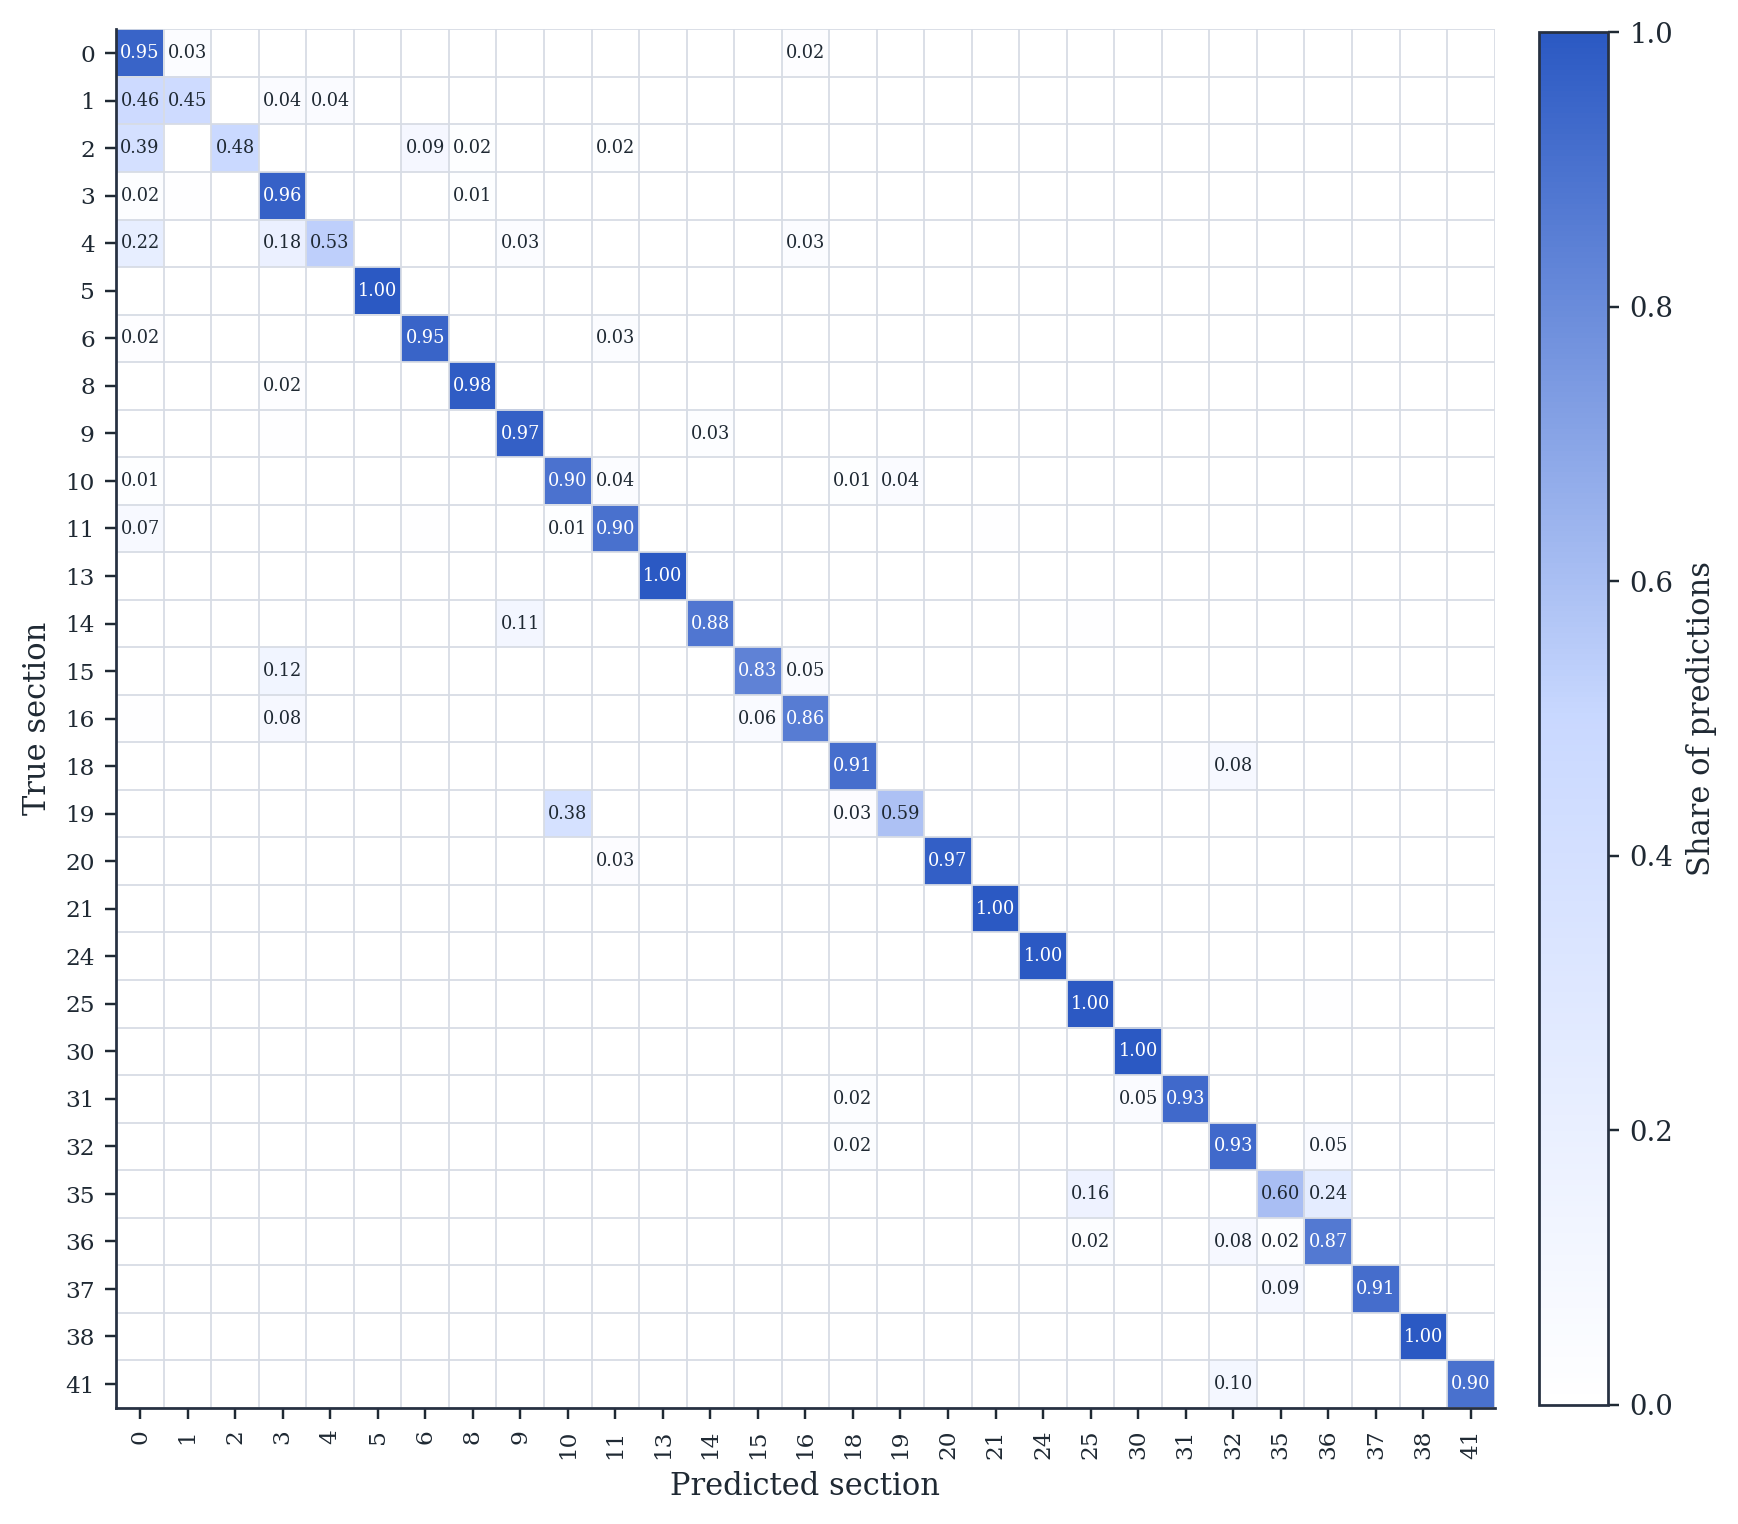
\includegraphics[width=15.5cm]{Figures/bwd_result_confusion_matrix_normalized.png}}
	\end{adjustwidth}
	\caption{Return-subnet diagnostics, excluding the "no defect" class: (\textbf{a}) distribution of predicted classes and (\textbf{b}) normalized confusion matrix.
		\label{fig:return_distribution_confusion}}
\end{figure}

\textcolor{blue}{The class-distribution panels in
Figures~\ref{fig:supply_distribution_confusion}
and~\ref{fig:return_distribution_confusion} should be interpreted as marginal
class-count diagnostics rather than as direct measures of class-wise
localization accuracy. In these panels, ``True'' denotes the number of test
samples whose simulated defect is located in the corresponding section, while
``Predicted Right'' and ``Predicted Wrong'' denote correct and incorrect
predictions assigned to that section, respectively.
Similar true and predicted counts can still hide
compensating errors between neighbouring sections. Therefore, the distribution
plots are considered together with the corresponding confusion matrices, which
show the actual class-to-class error structure.}

\textcolor{blue}{The distribution of predicted classes and the corresponding confusion matrices
in Figures~\ref{fig:supply_distribution_confusion}
and~\ref{fig:return_distribution_confusion} support
the earlier observations. For the supply subnet, the main errors are
concentrated in the remote group of segments 32, 36, and 41, with segment 41
being the most problematic case; this confirms that the model has difficulty
separating weak fault signatures in the farthest part of the network. For the return subnet, the
diffuse, scattered pattern of misclassifications across multiple classes
confirms that the narrower dynamic range makes fault signatures less
discriminative, and the noise begins to mask the underlying data patterns. In
particular, return-subnet segment 0 is often confused with nearby segments 1,
2, and 4. This segment is closest to the return-side sink and therefore lies
among the most distant sections from the source along the return path. As the
distance from the source increases, hydraulic and thermal responses become
smoother and defect signatures affect the measured parameters less explicitly.
Moreover, segment 0 contains several long pipes, so disturbances originating in
adjacent sections can produce similar aggregate signatures and be assigned to
segment 0.}

\subsection{Ablation Studies}

To validate our architectural choices, we conducted a comprehensive ablation
study examining three key aspects: (1) model depth and the impact of multi-head
attention mechanisms with skip connections, (2) pooling strategies, (3) number
of attention heads, and (4) choice of graph convolution layer type. All
experiments were performed on the fault classification task using the DHN
dataset described in Section \ref{stage2}.

As can be seen in Tables \ref{tab:ablation_depth},
\ref{tab:ablation_comprehensive}, the ablation experiments confirm our
hypothesis that the proposed architecture is optimal among comparable
alternatives, with the attention mechanism serving as a key factor in
prediction quality, both in the node encoder and as an edge-attention layer.
\begin{table}[H]
	\centering
	\begin{tabularx}{\textwidth}{lcccccc}
		\toprule
		\textbf{Configuration}         & \multicolumn{2}{c}{\textbf{S (4 layers)}} & \multicolumn{2}{c}{\textbf{M (8 layers)}} & \multicolumn{2}{c}{\textbf{L (16 layers)}}                 \\
		\cmidrule(lr){2-3} \cmidrule(lr){4-5} \cmidrule(lr){6-7}
		                               & Acc                                       & F1                                        & Acc                                        & F1 & Acc & F1 \\
		\midrule
		Attention + skip connections   & 91.4                                      & 86.8                                      &
		\textbf{92.1}                  & \textbf{ 87.6}                            & 73.5                                      & 30.0                                                       \\
		Attention w/o skip connections & 88.7                                      & 79.2                                      &
		\textbf{90.2}                  & \textbf{75.7}                             & 73.5                                      & 31.5                                                       \\
		No attention (MLP)             & 84.9                                      & 67.3                                      &
		\textbf{86.6}                  & \textbf{76.5}                             & 71.3                                      & 24.8                                                       \\
		\hline
		Number of parameters           & \multicolumn{2}{c}{725K}                  & \multicolumn{2}{c}{1.45M}                 & \multicolumn{2}{c}{2.9M}                                   \\
		\bottomrule
	\end{tabularx}
	\caption{Ablation study results: impact of model depth, multi-head attention mechanism, and skip connections on classification accuracy (\%) and macro F1-score (\%).}
	\label{tab:ablation_depth}
\end{table}

\begin{table}[H]
	\centering
	\begin{tabularx}{\textwidth}{lcc}
		\toprule
		\textbf{Configuration}  & \textbf{Accuracy (\%)} & \textbf{Macro F1 (\%)}                            \\
		\midrule
		\multicolumn{3}{l}{\textbf{Baseline: 8 layers, GATv2, attention + skip, 4 heads, attention pooling}} \\
		\midrule
		\multicolumn{3}{l}{\textbf{Pooling strategies}}                                                      \\
		\quad Attention pooling & \textbf{92.1}          & \textbf{87.6}                                     \\
		\quad Mean pooling      & 86.7                   & 65.9                                              \\
		\midrule
		\multicolumn{3}{l}{\textbf{Attention heads}}                                                         \\
		\quad 2 heads           & 88.7                   & 78.5                                              \\
		\quad 4 heads           & 92.1                   & 87.6                                              \\
		\quad 8 heads           & \textbf{93.6}          & \textbf{90.0}                                     \\
		\quad 16 heads          & 91.8                   & 86.1                                              \\
		\midrule
		\multicolumn{3}{l}{\textbf{Graph convolution layer types}}                                           \\
		\quad GATv2             & \textbf{92.1}          & \textbf{87.6}                                     \\
		\quad GraphSAGE         & 83.7                   & 52.6                                              \\
		\quad GCN               & 66.2                   & 16.6                                              \\
		\bottomrule
	\end{tabularx}
	\caption{Ablation study results on the 8-layer architecture with attention and skip connections.}
	\label{tab:ablation_comprehensive}
\end{table}

\textbf{Future Perspectives.}
While the unified architecture demonstrated robust performance, the observed discrepancy in accuracy between the supply ($0.960$) and return ($0.910$) subnets suggests that the current modeling approach may not fully capture the distinct hydraulic regimes. To address this, future work will explore a two-stage extension of the current framework.

First, we will assess the potential benefits of decoupling the networks by
training two distinct specialized models. This baseline experiment could help
establish the performance ceiling achievable by treating the supply and return
domains as separate learning problems. Furthermore, it may be beneficial to
implement graph-type conditioning, where the message-passing mechanism
explicitly utilizes different weight matrices for supply and return features.
Such an approach might allow the model to better distinguish the patterns in
data, potentially closing the accuracy gap while maintaining a single
deployable system.

%%%%%%%%%%%%%%%%%%%%%%%%%%%%%%%%%%%%%%%%%%
\section{Conclusions}

In this study, we addressed the challenge of fault localization in DHNs under
conditions of data scarcity, a common constraint in real-world infrastructure
monitoring. By using GNNs, we exploited the topological structure of DHNs to
overcome the limitations of traditional physics-based and topology-agnostic
data-driven methods.

The research was conducted in two distinct stages. First, we utilized a
synthetic dataset to identify an architecture capable of capturing long-range
dependencies in graph-structured data. This led to the design of a deep GNN
architecture integrating GATv2 node encoders and edge-attention mechanisms.
Second, we validated this architecture on a physically modeled dataset
generated via thermohydraulic simulations, representing a realistic urban
heating network.

The results demonstrated that the proposed model achieves high localization
accuracy on the test set: {96.0\%} for the supply subnet and {91.0\%} for the
return subnet, with corresponding Macro F1 scores of {93.0\%} and {86.9\%},
respectively. These metrics were obtained under sparse sensor coverage (only 30
of 187 nodes contained non-zero thermal and pressure features), simulating
realistic, data-limited conditions. The ablation studies further confirmed that
the attention mechanism and network depth are critical factors for performance.
The distance confusion matrix reveals that most errors are localized within a
topological distance of 1–2 sections from the actual defect. This confirms that
the model implicitly captures the attenuation of hydraulic and thermal
disturbances along the network topology.

\textcolor{blue}{The current thermohydraulic model is a simplified representation of a real district heating network. It does not include shut-off and control valves (e.g., gate valves, check valves, bypasses), intermediate switching states, or gradual pipe degradation. These factors will be incorporated in future work to reduce the simulation-to-reality gap.}

These findings suggest that topology-aware deep learning offers a promising
approach for DHN monitoring. Future work will focus on validating the approach
on historical field data from operational networks and testing it across
different district heating geometries and sensor layouts, while addressing the
inevitable domain shift between simulated training regimes and real-world
seasonal and load variations.

\textcolor{blue}{In practical predictive-maintenance workflows, the proposed
GNN can be used as an additional localization and ranking layer.
Standard-based risk estimates, pipe age and material data, pipe-static or
fatigue assessments, historical water-loss records, leakage-wire alarms, and
operating-history data can define prior fault probabilities, while the GNN uses
sparse SCADA-like pressure and temperature measurements together with network
topology to narrow the inspection area.}

However, we recognize that the most significant challenge remains the
acquisition of high-quality, labeled data to support such data-driven
methodologies.

%%%%%%%%%%%%%%%%%%%%%%%%%%%%%%%%%%%%%%%%%%

%%%%%%%%%%%%%%%%%%%%%%%%%%%%%%%%%%%%%%%%%%
% \section{Patents}

% This section is not mandatory, but may be added if there are patents resulting from the work reported in this manuscript.

%%%%%%%%%%%%%%%%%%%%%%%%%%%%%%%%%%%%%%%%%%
\vspace{6pt}

%%%%%%%%%%%%%%%%%%%%%%%%%%%%%%%%%%%%%%%%%%

\authorcontributions{Conceptualization, A.D. and R.M.; methodology, R.M. and O.G.; software, I.P. and S.F.; formal analysis, I.P. and D.P.; investigation, I.P. and D.P.; data curation, I.P. and S.F.; writing---original draft preparation, D.P.; writing---review and editing, I.P. and O.G.; visualization, I.P. and D.P.; supervision, S.A. and R.M. All authors have read and agreed to the published version of the manuscript.}

\funding{This work was supported by a grant for research centers, provided by the Ministry of Economic Development of the Russian Federation in accordance with the subsidy agreement with the Novosibirsk State University dated April 17, 2025 No. 139-15-2025-006: IGK 000000C313925P3S0002}

% \institutionalreview{In this section, you should add the Institutional Review Board Statement and approval number, if relevant to your study. You might choose to exclude this statement if the study did not require ethical approval. Please note that the Editorial Office might ask you for further information. Please add “The study was conducted in accordance with the Declaration of Helsinki, and approved by the Institutional Review Board (or Ethics Committee) of NAME OF INSTITUTE (protocol code XXX and date of approval).” for studies involving humans. OR “The animal study protocol was approved by the Institutional Review Board (or Ethics Committee) of NAME OF INSTITUTE (protocol code XXX and date of approval).” for studies involving animals. OR “Ethical review and approval were waived for this study due to REASON (please provide a detailed justification).” OR “Not applicable” for studies not involving humans or animals.}

%\informedconsent{Any research article describing a study involving humans should contain this statement. Please add ``Informed consent was obtained from all subjects involved in the study.'' OR ``Patient consent was waived due to REASON (please provide a detailed justification).'' OR ``Not applicable'' for studies not involving humans. You might also choose to exclude this statement if the study did not involve humans.

%Written informed consent for publication must be obtained from participating patients who can be identified (including by the patients themselves). Please state ``Written informed consent has been obtained from the patient(s) to publish this paper'' if applicable.}

\dataavailability{All data are available on request from the corresponding authors.}

%\dataavailability{We encourage all authors of articles published in MDPI journals to share their research data. In this section, please provide details regarding where data supporting reported results can be found, including links to publicly archived datasets analyzed or generated during the study. Where no new data were created, or where data is unavailable due to privacy or ethical restrictions, a statement is still required. Suggested Data Availability Statements are available in section ``MDPI Research Data Policies'' at \url{https://www.mdpi.com/ethics}.} 

%\durcstatement{Current research is limited to the [please insert a specific academic field, e.g., XXX], which is beneficial [share benefits and/or primary use] and does not pose a threat to public health or national security. Authors acknowledge the dual-use potential of the research involving xxx and confirm that all necessary precautions have been taken to prevent potential misuse. As an ethical responsibility, authors strictly adhere to relevant national and international laws about DURC. Authors advocate for responsible deployment, ethical considerations, regulatory compliance, and transparent reporting to mitigate misuse risks and foster beneficial outcomes.}

%\acknowledgments{In this section you can acknowledge any support given which is not covered by the author contribution or funding sections. This may include administrative and technical support, or donations in kind (e.g., materials used for experiments). Where GenAI has been used for purposes such as generating text, data, or graphics, or for study design, data collection, analysis, or interpretation of data, please add “During the preparation of this manuscript/study, the author(s) used [tool name, version information] for the purposes of [description of use]. The authors have reviewed and edited the output and take full responsibility for the content of this publication.”}

\conflictsofinterest{The authors declare no conflicts of interest.}

%%%%%%%%%%%%%%%%%%%%%%%%%%%%%%%%%%%%%%%%%%
%% Optional

%% Only for journal Encyclopedia
%\entrylink{The Link to this entry published on the encyclopedia platform.}

\abbreviations{Abbreviations}{
	The following abbreviations are used in this manuscript:
	\\
	\noindent
	\begin{tabular}{@{}ll}
		CGNN      & Composite Graph Neural Network                     \\
		CNN       & Convolutional Neural Network                       \\
		DHN       & District Heating Network                           \\
		GAT       & Graph Attention Network                            \\
		GCN       & Graph Convolutional Network                        \\
		GNN       & Graph Neural Network                               \\
		GraphSAGE & Graph SAmple and aggreGatE                         \\
		ReLU      & Rectified Linear Unit                              \\
		SCADA     & Supervisory Control and Data Acquisition           \\
		SIMPLE    & Semi-Implicit Method for Pressure-Linked Equations \\
		SVM       & Support Vector Machine                             \\
		UAV       & Unmanned Aerial Vehicle                            \\
	\end{tabular}
}

\abbreviations{Nomenclature}{

	\noindent
	\begin{tabular}{@{}ll}
		$A$            & Cross-sectional area of the pipe                             \\
		$c_p$          & Specific heat capacity of the fluid                          \\
		$d$            & Distance metric                                              \\
		$e$            & Graph edge                                                   \\
		$F$            & Surface area of the pipe                                     \\
		$f_k(e)$       & Target variable function for edge $e$                        \\
		$k$            & Number of hops (neighborhood radius)                         \\
		$m_l$          & Mass flow rate vector along the connected edges              \\
		$N_k(e)$       & Set of nodes within a $k$-hop neighborhood of edge $e$       \\
		$p$            & Pressure                                                     \\
		$p'$           & Pressure correction                                          \\
		$P$            & Set of edges in the shortest path between nodes              \\
		$q$            & Mass source or sink at the specific node                     \\
		$Q$            & Heat loss from pipe to ambient air                           \\
		$s$            & Hydraulic resistance coefficient                             \\
		$t_1$          & Inlet temperature                                            \\
		$t_b$          & Average water temperature within the pipe                    \\
		$t_{out}$      & Ambient outdoor temperature                                  \\
		$t_i$          & Nodal temperature                                            \\
		$u_b$          & Flow velocity                                                \\
		$W_i$          & Edge feature                                                 \\
		$X_i$          & Node attribute                                               \\
		$\alpha$       & Overall heat transfer coefficient                            \\
		$\Delta p$     & Pressure drop over the pipe                                  \\
		$\kappa$       & Coefficient derived from hydraulic resistance ($1/(s|m_l|)$) \\
		$\lambda$      & Decay factor                                                 \\
		$\rho$         & Fluid density                                                \\
		$\nabla \cdot$ & Divergence operator                                          \\
	\end{tabular}
}

%%%%%%%%%%%%%%%%%%%%%%%%%%%%%%%%%%%%%%%%%%
%% Optional
% \appendixtitles{no} % Leave argument "no" if all appendix headings stay EMPTY (then no dot is printed after "Appendix A"). If the appendix sections contain a heading then change the argument to "yes".
% \appendixstart
% \appendix
% \section[\appendixname~\thesection]{}
% \subsection[\appendixname~\thesubsection]{}
% The appendix is an optional section that can contain details and data supplemental to the main text---for example, explanations of experimental details that would disrupt the flow of the main text but nonetheless remain crucial to understanding and reproducing the research shown; figures of replicates for experiments of which representative data are shown in the main text can be added here if brief, or as Supplementary Data. Mathematical proofs of results not central to the paper can be added as an appendix.

% \begin{table}[H] 
% \caption{This is a table caption.\label{tab5}}
% %\newcolumntype{C}{>{\centering\arraybackslash}X}
% \begin{tabularx}{\textwidth}{CCC}
% \toprule
% \textbf{Title 1}	& \textbf{Title 2}	& \textbf{Title 3}\\
% \midrule
% Entry 1		& Data			& Data\\
% Entry 2		& Data			& Data\\
% \bottomrule
% \end{tabularx}
% \end{table}

% \section[\appendixname~\thesection]{}
% All appendix sections must be cited in the main text. In the appendices, Figures, Tables, etc. should be labeled, starting with ``A''---e.g., Figure A1, Figure A2, etc.

%%%%%%%%%%%%%%%%%%%%%%%%%%%%%%%%%%%%%%%%%%
%\isPreprints{}{% This command is only used for ``preprints''.
\begin{adjustwidth}{-\extralength}{0cm}
	%} % If the paper is ``preprints'', please uncomment this parenthesis.
	%\printendnotes[custom] % Un-comment to print a list of endnotes

	\reftitle{References}

	% Please provide either the correct journal abbreviation (e.g. according to the “List of Title Word Abbreviations” http://www.issn.org/services/online-services/access-to-the-ltwa/) or the full name of the journal.
	% Citations and References in Supplementary files are permitted provided that they also appear in the reference list here. 

	%=====================================
	% References, variant A: external bibliography
	%=====================================
	\bibliography{bibliography}

	%=====================================
	% References, variant B: internal bibliography
	%=====================================

	% If authors have biography, please use the format below
	%\section*{Short Biography of Authors}
	%\bio
	%{\raisebox{-0.35cm}{\includegraphics[width=3.5cm,height=5.3cm,clip,keepaspectratio]{Definitions/author1.pdf}}}
	%{\textbf{Firstname Lastname} Biography of first author}
	%
	%\bio
	%{\raisebox{-0.35cm}{\includegraphics[width=3.5cm,height=5.3cm,clip,keepaspectratio]{Definitions/author2.jpg}}}
	%{\textbf{Firstname Lastname} Biography of second author}

	% For the MDPI journals use author-date citation, please follow the formatting guidelines on http://www.mdpi.com/authors/references
	% To cite two works by the same author: \citeauthor{ref-journal-1a} (\citeyear{ref-journal-1a}, \citeyear{ref-journal-1b}). This produces: Whittaker (1967, 1975)
	% To cite two works by the same author with specific pages: \citeauthor{ref-journal-3a} (\citeyear{ref-journal-3a}, p. 328; \citeyear{ref-journal-3b}, p.475). This produces: Wong (1999, p. 328; 2000, p. 475)

	%%%%%%%%%%%%%%%%%%%%%%%%%%%%%%%%%%%%%%%%%%
	%% for journal Sci
	%\reviewreports{\\
	%Reviewer 1 comments and authors’ response\\
	%Reviewer 2 comments and authors’ response\\
	%Reviewer 3 comments and authors’ response
	%}
	%%%%%%%%%%%%%%%%%%%%%%%%%%%%%%%%%%%%%%%%%%
	\PublishersNote{}
	%\isPreprints{}{% This command is only used for ``preprints''.
\end{adjustwidth}
%} % If the paper is ``preprints'', please uncomment this parenthesis.
\end{document}
